% !TeX program = xelatex
% Prezentacija (Beamer) - minimalistička, bela pozadina, srpski (latinica)
% Zasnovano na diplomskom radu "Fraktal renderovanje sa hibridnom paralelizacijom"
% Ciljano trajanje: 12-16 minuta, ~1 minut po slajdu (16 slajdova)
% Kompajliranje:  xelatex main.tex   (dva puta, zbog brojača strana)

\documentclass[aspectratio=169,11pt]{beamer}

\usepackage{fontspec}
\usepackage{polyglossia}
\setmainlanguage[script=latin]{serbian}
\setmainfont{Inter}
\setmonofont{DejaVu Sans Mono}[Scale=0.86]

\usepackage{amsmath}
\usepackage{amssymb}
\usepackage{graphicx}
\usepackage{tikz}
\usetikzlibrary{arrows.meta,positioning,fit,shapes.geometric}
\usepackage{booktabs}

%% ------------------------------------------------------------------
%% Boje - minimalistička paleta: bela pozadina, jedan akcenat
%% ------------------------------------------------------------------
\definecolor{accent}{HTML}{1B4B66}
\definecolor{accentlight}{HTML}{5C8AA6}
\definecolor{accentwarm}{HTML}{C1601E}
\definecolor{darktext}{HTML}{202020}
\definecolor{graytext}{HTML}{707070}
\definecolor{palegray}{HTML}{E7E7E7}

\setbeamertemplate{navigation symbols}{}
\setbeamercolor{background canvas}{bg=white}
\setbeamercolor{normal text}{fg=darktext,bg=white}
\setbeamercolor{structure}{fg=accent}
\setbeamercolor{title}{fg=accent,bg=white}
\setbeamercolor{frametitle}{fg=accent,bg=white}
\setbeamercolor{itemize item}{fg=accent}
\setbeamercolor{itemize subitem}{fg=accentlight}
\setbeamercolor{footline}{fg=graytext,bg=white}
\setbeamercolor{caption}{fg=graytext}
\setbeamercolor{block title}{fg=accent,bg=palegray}
\setbeamercolor{block body}{fg=darktext,bg=white}

\setbeamerfont{title}{size=\huge,series=\bfseries}
\setbeamerfont{frametitle}{size=\Large,series=\bfseries}
\setbeamerfont{caption}{size=\scriptsize}

\setbeamertemplate{itemize item}{\textcolor{accent}{\scriptsize\raisebox{0.15ex}{$\blacktriangleright$}}}
\setbeamertemplate{itemize subitem}{\textcolor{accentlight}{\textendash}}
\setbeamertemplate{enumerate item}{\textcolor{accent}{\bfseries\insertenumlabel.}}

\setbeamertemplate{frametitle}{%
  \vskip0.5em%
  {\usebeamerfont{frametitle}\usebeamercolor[fg]{frametitle}\insertframetitle}\par%
  \vskip0.3em%
  {\color{accent}\hrule height 0.9pt}%
  \vskip0.45em%
}

\setbeamertemplate{footline}{%
  \begin{beamercolorbox}[wd=\paperwidth,ht=2.6ex,dp=1.4ex,right,rightskip=0.9em plus1fil,leftskip=0.9em]{footline}
    {\color{graytext}\scriptsize Fraktal renderovanje sa hibridnom paralelizacijom \hfill \insertframenumber\,/\,\inserttotalframenumber}
  \end{beamercolorbox}
}

\newcommand{\code}[1]{\texttt{\color{accent!80!black}#1}}

\title{Fraktal renderovanje sa hibridnom paralelizacijom}
\author{Tamaš Pap}
\date{2026}

\begin{document}

%% ==================================================================== 1
\begin{frame}[plain]
  \vspace{-0.3cm}
  \begin{center}
    
\includegraphics[height=1.35cm]{figures/ftn-logo.png}\\[0.6em]
    {\color{accent}\rule{0.16\textwidth}{2pt}}\\[0.9em]
    {\usebeamerfont{title}\color{accent} Fraktal renderovanje sa\\[0.15em] hibridnom paralelizacijom}\\[1em]
    {\large\color{graytext} Diplomski rad}\\[1.6em]
    {\large\color{darktext} Tamaš Pap}\\[0.35em]
    {\small\color{graytext} Mentor: dr Veljko Petrović}\\[1.6em]
    {\small\color{graytext}
      Fakultet tehničkih nauka, Novi Sad\\
      Računarstvo i automatika\\
      2026}
  \end{center}
\end{frame}

%% ==================================================================== 1b
\begin{frame}{Šta su fraktali i čemu služe?}
  \vspace{-0.2cm}
  \begin{columns}[T]
    \column{0.52\textwidth}
      \footnotesize
      \begin{itemize}
        \item Oblik čija se složenost \textbf{ne gubi uvećanjem} i koji je samosličan, sa fraktalnom dimenzijom koja nije ceo broj
        \item U prirodi: obalske linije, rečne mreže, oblaci, otkucaji srca, pluća i krvni sudovi (grananje)
      \end{itemize}
      \vspace{0.15em}
      \textbf{Čemu služe:}
      \begin{itemize}
        \item kompresija slike (iterirani sistemi funkcija)
        \item kompaktne fraktalne antene za rad na više frekvencija
        \item proceduralna grafika (teren, oblaci, teksture)
        \item dijagnostika u medicini: fraktalna dimenzija tkiva i krvnih sudova razlikuje zdravo od obolelog
      \end{itemize}
      \normalsize
    \column{0.44\textwidth}
      \centering
      \begin{tikzpicture}[x=1.8cm,y=1.8cm]
        \begin{scope}
          \clip (0,0) rectangle (1,0.4);
          \draw[thick] plot coordinates {(0.00000,0.00000) (0.01235,0.00000) (0.01852,0.01069) (0.02469,0.00000) (0.03704,0.00000) (0.04321,0.01069) (0.03704,0.02138) (0.04938,0.02138) (0.05556,0.03208) (0.06173,0.02138) (0.07407,0.02138) (0.06790,0.01069) (0.07407,0.00000) (0.08642,0.00000) (0.09259,0.01069) (0.09877,0.00000) (0.11111,0.00000) (0.11728,0.01069) (0.11111,0.02138) (0.12346,0.02138) (0.12963,0.03208) (0.12346,0.04277) (0.11111,0.04277) (0.11728,0.05346) (0.11111,0.06415) (0.12346,0.06415) (0.12963,0.07484) (0.13580,0.06415) (0.14815,0.06415) (0.15432,0.07484) (0.14815,0.08553) (0.16049,0.08553) (0.16667,0.09623) (0.17284,0.08553) (0.18519,0.08553) (0.17901,0.07484) (0.18519,0.06415) (0.19753,0.06415) (0.20370,0.07484) (0.20988,0.06415) (0.22222,0.06415) (0.21605,0.05346) (0.22222,0.04277) (0.20988,0.04277) (0.20370,0.03208) (0.20988,0.02138) (0.22222,0.02138) (0.21605,0.01069) (0.22222,0.00000) (0.23457,0.00000) (0.24074,0.01069) (0.24691,0.00000) (0.25926,0.00000) (0.26543,0.01069) (0.25926,0.02138) (0.27160,0.02138) (0.27778,0.03208) (0.28395,0.02138) (0.29630,0.02138) (0.29012,0.01069) (0.29630,0.00000) (0.30864,0.00000) (0.31481,0.01069) (0.32099,0.00000) (0.33333,0.00000) (0.33951,0.01069) (0.33333,0.02138) (0.34568,0.02138) (0.35185,0.03208) (0.34568,0.04277) (0.33333,0.04277) (0.33951,0.05346) (0.33333,0.06415) (0.34568,0.06415) (0.35185,0.07484) (0.35802,0.06415) (0.37037,0.06415) (0.37654,0.07484) (0.37037,0.08553) (0.38272,0.08553) (0.38889,0.09623) (0.38272,0.10692) (0.37037,0.10692) (0.37654,0.11761) (0.37037,0.12830) (0.35802,0.12830) (0.35185,0.11761) (0.34568,0.12830) (0.33333,0.12830) (0.33951,0.13899) (0.33333,0.14968) (0.34568,0.14968) (0.35185,0.16038) (0.34568,0.17107) (0.33333,0.17107) (0.33951,0.18176) (0.33333,0.19245) (0.34568,0.19245) (0.35185,0.20314) (0.35802,0.19245) (0.37037,0.19245) (0.37654,0.20314) (0.37037,0.21383) (0.38272,0.21383) (0.38889,0.22453) (0.39506,0.21383) (0.40741,0.21383) (0.40123,0.20314) (0.40741,0.19245) (0.41975,0.19245) (0.42593,0.20314) (0.43210,0.19245) (0.44444,0.19245) (0.45062,0.20314) (0.44444,0.21383) (0.45679,0.21383) (0.46296,0.22453) (0.45679,0.23522) (0.44444,0.23522) (0.45062,0.24591) (0.44444,0.25660) (0.45679,0.25660) (0.46296,0.26729) (0.46914,0.25660) (0.48148,0.25660) (0.48765,0.26729) (0.48148,0.27798) (0.49383,0.27798) (0.50000,0.28868) (0.50617,0.27798) (0.51852,0.27798) (0.51235,0.26729) (0.51852,0.25660) (0.53086,0.25660) (0.53704,0.26729) (0.54321,0.25660) (0.55556,0.25660) (0.54938,0.24591) (0.55556,0.23522) (0.54321,0.23522) (0.53704,0.22453) (0.54321,0.21383) (0.55556,0.21383) (0.54938,0.20314) (0.55556,0.19245) (0.56790,0.19245) (0.57407,0.20314) (0.58025,0.19245) (0.59259,0.19245) (0.59877,0.20314) (0.59259,0.21383) (0.60494,0.21383) (0.61111,0.22453) (0.61728,0.21383) (0.62963,0.21383) (0.62346,0.20314) (0.62963,0.19245) (0.64198,0.19245) (0.64815,0.20314) (0.65432,0.19245) (0.66667,0.19245) (0.66049,0.18176) (0.66667,0.17107) (0.65432,0.17107) (0.64815,0.16038) (0.65432,0.14968) (0.66667,0.14968) (0.66049,0.13899) (0.66667,0.12830) (0.65432,0.12830) (0.64815,0.11761) (0.64198,0.12830) (0.62963,0.12830) (0.62346,0.11761) (0.62963,0.10692) (0.61728,0.10692) (0.61111,0.09623) (0.61728,0.08553) (0.62963,0.08553) (0.62346,0.07484) (0.62963,0.06415) (0.64198,0.06415) (0.64815,0.07484) (0.65432,0.06415) (0.66667,0.06415) (0.66049,0.05346) (0.66667,0.04277) (0.65432,0.04277) (0.64815,0.03208) (0.65432,0.02138) (0.66667,0.02138) (0.66049,0.01069) (0.66667,0.00000) (0.67901,0.00000) (0.68519,0.01069) (0.69136,0.00000) (0.70370,0.00000) (0.70988,0.01069) (0.70370,0.02138) (0.71605,0.02138) (0.72222,0.03208) (0.72840,0.02138) (0.74074,0.02138) (0.73457,0.01069) (0.74074,0.00000) (0.75309,0.00000) (0.75926,0.01069) (0.76543,0.00000) (0.77778,0.00000) (0.78395,0.01069) (0.77778,0.02138) (0.79012,0.02138) (0.79630,0.03208) (0.79012,0.04277) (0.77778,0.04277) (0.78395,0.05346) (0.77778,0.06415) (0.79012,0.06415) (0.79630,0.07484) (0.80247,0.06415) (0.81481,0.06415) (0.82099,0.07484) (0.81481,0.08553) (0.82716,0.08553) (0.83333,0.09623) (0.83951,0.08553) (0.85185,0.08553) (0.84568,0.07484) (0.85185,0.06415) (0.86420,0.06415) (0.87037,0.07484) (0.87654,0.06415) (0.88889,0.06415) (0.88272,0.05346) (0.88889,0.04277) (0.87654,0.04277) (0.87037,0.03208) (0.87654,0.02138) (0.88889,0.02138) (0.88272,0.01069) (0.88889,0.00000) (0.90123,0.00000) (0.90741,0.01069) (0.91358,0.00000) (0.92593,0.00000) (0.93210,0.01069) (0.92593,0.02138) (0.93827,0.02138) (0.94444,0.03208) (0.95062,0.02138) (0.96296,0.02138) (0.95679,0.01069) (0.96296,0.00000) (0.97531,0.00000) (0.98148,0.01069) (0.98765,0.00000) (1.00000,0.00000)};

        \end{scope}
      \end{tikzpicture}\\[0.05em]
      {\scriptsize\color{graytext} Kohova kriva}\\[0.5em]
      \begin{tikzpicture}[x=1.2cm,y=1.2cm]
        \fill (0.00000,0.00000) -- (0.03125,0.00000) -- (0.01562,0.02706) -- cycle;
\fill (0.03125,0.00000) -- (0.06250,0.00000) -- (0.04688,0.02706) -- cycle;
\fill (0.01562,0.02706) -- (0.04688,0.02706) -- (0.03125,0.05413) -- cycle;
\fill (0.06250,0.00000) -- (0.09375,0.00000) -- (0.07812,0.02706) -- cycle;
\fill (0.09375,0.00000) -- (0.12500,0.00000) -- (0.10938,0.02706) -- cycle;
\fill (0.07812,0.02706) -- (0.10938,0.02706) -- (0.09375,0.05413) -- cycle;
\fill (0.03125,0.05413) -- (0.06250,0.05413) -- (0.04688,0.08119) -- cycle;
\fill (0.06250,0.05413) -- (0.09375,0.05413) -- (0.07812,0.08119) -- cycle;
\fill (0.04688,0.08119) -- (0.07812,0.08119) -- (0.06250,0.10825) -- cycle;
\fill (0.12500,0.00000) -- (0.15625,0.00000) -- (0.14062,0.02706) -- cycle;
\fill (0.15625,0.00000) -- (0.18750,0.00000) -- (0.17188,0.02706) -- cycle;
\fill (0.14062,0.02706) -- (0.17188,0.02706) -- (0.15625,0.05413) -- cycle;
\fill (0.18750,0.00000) -- (0.21875,0.00000) -- (0.20312,0.02706) -- cycle;
\fill (0.21875,0.00000) -- (0.25000,0.00000) -- (0.23438,0.02706) -- cycle;
\fill (0.20312,0.02706) -- (0.23438,0.02706) -- (0.21875,0.05413) -- cycle;
\fill (0.15625,0.05413) -- (0.18750,0.05413) -- (0.17188,0.08119) -- cycle;
\fill (0.18750,0.05413) -- (0.21875,0.05413) -- (0.20312,0.08119) -- cycle;
\fill (0.17188,0.08119) -- (0.20312,0.08119) -- (0.18750,0.10825) -- cycle;
\fill (0.06250,0.10825) -- (0.09375,0.10825) -- (0.07812,0.13532) -- cycle;
\fill (0.09375,0.10825) -- (0.12500,0.10825) -- (0.10938,0.13532) -- cycle;
\fill (0.07812,0.13532) -- (0.10938,0.13532) -- (0.09375,0.16238) -- cycle;
\fill (0.12500,0.10825) -- (0.15625,0.10825) -- (0.14062,0.13532) -- cycle;
\fill (0.15625,0.10825) -- (0.18750,0.10825) -- (0.17188,0.13532) -- cycle;
\fill (0.14062,0.13532) -- (0.17188,0.13532) -- (0.15625,0.16238) -- cycle;
\fill (0.09375,0.16238) -- (0.12500,0.16238) -- (0.10938,0.18944) -- cycle;
\fill (0.12500,0.16238) -- (0.15625,0.16238) -- (0.14062,0.18944) -- cycle;
\fill (0.10938,0.18944) -- (0.14062,0.18944) -- (0.12500,0.21651) -- cycle;
\fill (0.25000,0.00000) -- (0.28125,0.00000) -- (0.26562,0.02706) -- cycle;
\fill (0.28125,0.00000) -- (0.31250,0.00000) -- (0.29688,0.02706) -- cycle;
\fill (0.26562,0.02706) -- (0.29688,0.02706) -- (0.28125,0.05413) -- cycle;
\fill (0.31250,0.00000) -- (0.34375,0.00000) -- (0.32812,0.02706) -- cycle;
\fill (0.34375,0.00000) -- (0.37500,0.00000) -- (0.35938,0.02706) -- cycle;
\fill (0.32812,0.02706) -- (0.35938,0.02706) -- (0.34375,0.05413) -- cycle;
\fill (0.28125,0.05413) -- (0.31250,0.05413) -- (0.29688,0.08119) -- cycle;
\fill (0.31250,0.05413) -- (0.34375,0.05413) -- (0.32812,0.08119) -- cycle;
\fill (0.29688,0.08119) -- (0.32812,0.08119) -- (0.31250,0.10825) -- cycle;
\fill (0.37500,0.00000) -- (0.40625,0.00000) -- (0.39062,0.02706) -- cycle;
\fill (0.40625,0.00000) -- (0.43750,0.00000) -- (0.42188,0.02706) -- cycle;
\fill (0.39062,0.02706) -- (0.42188,0.02706) -- (0.40625,0.05413) -- cycle;
\fill (0.43750,0.00000) -- (0.46875,0.00000) -- (0.45312,0.02706) -- cycle;
\fill (0.46875,0.00000) -- (0.50000,0.00000) -- (0.48438,0.02706) -- cycle;
\fill (0.45312,0.02706) -- (0.48438,0.02706) -- (0.46875,0.05413) -- cycle;
\fill (0.40625,0.05413) -- (0.43750,0.05413) -- (0.42188,0.08119) -- cycle;
\fill (0.43750,0.05413) -- (0.46875,0.05413) -- (0.45312,0.08119) -- cycle;
\fill (0.42188,0.08119) -- (0.45312,0.08119) -- (0.43750,0.10825) -- cycle;
\fill (0.31250,0.10825) -- (0.34375,0.10825) -- (0.32812,0.13532) -- cycle;
\fill (0.34375,0.10825) -- (0.37500,0.10825) -- (0.35938,0.13532) -- cycle;
\fill (0.32812,0.13532) -- (0.35938,0.13532) -- (0.34375,0.16238) -- cycle;
\fill (0.37500,0.10825) -- (0.40625,0.10825) -- (0.39062,0.13532) -- cycle;
\fill (0.40625,0.10825) -- (0.43750,0.10825) -- (0.42188,0.13532) -- cycle;
\fill (0.39062,0.13532) -- (0.42188,0.13532) -- (0.40625,0.16238) -- cycle;
\fill (0.34375,0.16238) -- (0.37500,0.16238) -- (0.35938,0.18944) -- cycle;
\fill (0.37500,0.16238) -- (0.40625,0.16238) -- (0.39062,0.18944) -- cycle;
\fill (0.35938,0.18944) -- (0.39062,0.18944) -- (0.37500,0.21651) -- cycle;
\fill (0.12500,0.21651) -- (0.15625,0.21651) -- (0.14062,0.24357) -- cycle;
\fill (0.15625,0.21651) -- (0.18750,0.21651) -- (0.17188,0.24357) -- cycle;
\fill (0.14062,0.24357) -- (0.17188,0.24357) -- (0.15625,0.27063) -- cycle;
\fill (0.18750,0.21651) -- (0.21875,0.21651) -- (0.20312,0.24357) -- cycle;
\fill (0.21875,0.21651) -- (0.25000,0.21651) -- (0.23438,0.24357) -- cycle;
\fill (0.20312,0.24357) -- (0.23438,0.24357) -- (0.21875,0.27063) -- cycle;
\fill (0.15625,0.27063) -- (0.18750,0.27063) -- (0.17188,0.29770) -- cycle;
\fill (0.18750,0.27063) -- (0.21875,0.27063) -- (0.20312,0.29770) -- cycle;
\fill (0.17188,0.29770) -- (0.20312,0.29770) -- (0.18750,0.32476) -- cycle;
\fill (0.25000,0.21651) -- (0.28125,0.21651) -- (0.26562,0.24357) -- cycle;
\fill (0.28125,0.21651) -- (0.31250,0.21651) -- (0.29688,0.24357) -- cycle;
\fill (0.26562,0.24357) -- (0.29688,0.24357) -- (0.28125,0.27063) -- cycle;
\fill (0.31250,0.21651) -- (0.34375,0.21651) -- (0.32812,0.24357) -- cycle;
\fill (0.34375,0.21651) -- (0.37500,0.21651) -- (0.35938,0.24357) -- cycle;
\fill (0.32812,0.24357) -- (0.35938,0.24357) -- (0.34375,0.27063) -- cycle;
\fill (0.28125,0.27063) -- (0.31250,0.27063) -- (0.29688,0.29770) -- cycle;
\fill (0.31250,0.27063) -- (0.34375,0.27063) -- (0.32812,0.29770) -- cycle;
\fill (0.29688,0.29770) -- (0.32812,0.29770) -- (0.31250,0.32476) -- cycle;
\fill (0.18750,0.32476) -- (0.21875,0.32476) -- (0.20312,0.35182) -- cycle;
\fill (0.21875,0.32476) -- (0.25000,0.32476) -- (0.23438,0.35182) -- cycle;
\fill (0.20312,0.35182) -- (0.23438,0.35182) -- (0.21875,0.37889) -- cycle;
\fill (0.25000,0.32476) -- (0.28125,0.32476) -- (0.26562,0.35182) -- cycle;
\fill (0.28125,0.32476) -- (0.31250,0.32476) -- (0.29688,0.35182) -- cycle;
\fill (0.26562,0.35182) -- (0.29688,0.35182) -- (0.28125,0.37889) -- cycle;
\fill (0.21875,0.37889) -- (0.25000,0.37889) -- (0.23438,0.40595) -- cycle;
\fill (0.25000,0.37889) -- (0.28125,0.37889) -- (0.26562,0.40595) -- cycle;
\fill (0.23438,0.40595) -- (0.26562,0.40595) -- (0.25000,0.43301) -- cycle;
\fill (0.50000,0.00000) -- (0.53125,0.00000) -- (0.51562,0.02706) -- cycle;
\fill (0.53125,0.00000) -- (0.56250,0.00000) -- (0.54688,0.02706) -- cycle;
\fill (0.51562,0.02706) -- (0.54688,0.02706) -- (0.53125,0.05413) -- cycle;
\fill (0.56250,0.00000) -- (0.59375,0.00000) -- (0.57812,0.02706) -- cycle;
\fill (0.59375,0.00000) -- (0.62500,0.00000) -- (0.60938,0.02706) -- cycle;
\fill (0.57812,0.02706) -- (0.60938,0.02706) -- (0.59375,0.05413) -- cycle;
\fill (0.53125,0.05413) -- (0.56250,0.05413) -- (0.54688,0.08119) -- cycle;
\fill (0.56250,0.05413) -- (0.59375,0.05413) -- (0.57812,0.08119) -- cycle;
\fill (0.54688,0.08119) -- (0.57812,0.08119) -- (0.56250,0.10825) -- cycle;
\fill (0.62500,0.00000) -- (0.65625,0.00000) -- (0.64062,0.02706) -- cycle;
\fill (0.65625,0.00000) -- (0.68750,0.00000) -- (0.67188,0.02706) -- cycle;
\fill (0.64062,0.02706) -- (0.67188,0.02706) -- (0.65625,0.05413) -- cycle;
\fill (0.68750,0.00000) -- (0.71875,0.00000) -- (0.70312,0.02706) -- cycle;
\fill (0.71875,0.00000) -- (0.75000,0.00000) -- (0.73438,0.02706) -- cycle;
\fill (0.70312,0.02706) -- (0.73438,0.02706) -- (0.71875,0.05413) -- cycle;
\fill (0.65625,0.05413) -- (0.68750,0.05413) -- (0.67188,0.08119) -- cycle;
\fill (0.68750,0.05413) -- (0.71875,0.05413) -- (0.70312,0.08119) -- cycle;
\fill (0.67188,0.08119) -- (0.70312,0.08119) -- (0.68750,0.10825) -- cycle;
\fill (0.56250,0.10825) -- (0.59375,0.10825) -- (0.57812,0.13532) -- cycle;
\fill (0.59375,0.10825) -- (0.62500,0.10825) -- (0.60938,0.13532) -- cycle;
\fill (0.57812,0.13532) -- (0.60938,0.13532) -- (0.59375,0.16238) -- cycle;
\fill (0.62500,0.10825) -- (0.65625,0.10825) -- (0.64062,0.13532) -- cycle;
\fill (0.65625,0.10825) -- (0.68750,0.10825) -- (0.67188,0.13532) -- cycle;
\fill (0.64062,0.13532) -- (0.67188,0.13532) -- (0.65625,0.16238) -- cycle;
\fill (0.59375,0.16238) -- (0.62500,0.16238) -- (0.60938,0.18944) -- cycle;
\fill (0.62500,0.16238) -- (0.65625,0.16238) -- (0.64062,0.18944) -- cycle;
\fill (0.60938,0.18944) -- (0.64062,0.18944) -- (0.62500,0.21651) -- cycle;
\fill (0.75000,0.00000) -- (0.78125,0.00000) -- (0.76562,0.02706) -- cycle;
\fill (0.78125,0.00000) -- (0.81250,0.00000) -- (0.79688,0.02706) -- cycle;
\fill (0.76562,0.02706) -- (0.79688,0.02706) -- (0.78125,0.05413) -- cycle;
\fill (0.81250,0.00000) -- (0.84375,0.00000) -- (0.82812,0.02706) -- cycle;
\fill (0.84375,0.00000) -- (0.87500,0.00000) -- (0.85938,0.02706) -- cycle;
\fill (0.82812,0.02706) -- (0.85938,0.02706) -- (0.84375,0.05413) -- cycle;
\fill (0.78125,0.05413) -- (0.81250,0.05413) -- (0.79688,0.08119) -- cycle;
\fill (0.81250,0.05413) -- (0.84375,0.05413) -- (0.82812,0.08119) -- cycle;
\fill (0.79688,0.08119) -- (0.82812,0.08119) -- (0.81250,0.10825) -- cycle;
\fill (0.87500,0.00000) -- (0.90625,0.00000) -- (0.89062,0.02706) -- cycle;
\fill (0.90625,0.00000) -- (0.93750,0.00000) -- (0.92188,0.02706) -- cycle;
\fill (0.89062,0.02706) -- (0.92188,0.02706) -- (0.90625,0.05413) -- cycle;
\fill (0.93750,0.00000) -- (0.96875,0.00000) -- (0.95312,0.02706) -- cycle;
\fill (0.96875,0.00000) -- (1.00000,0.00000) -- (0.98438,0.02706) -- cycle;
\fill (0.95312,0.02706) -- (0.98438,0.02706) -- (0.96875,0.05413) -- cycle;
\fill (0.90625,0.05413) -- (0.93750,0.05413) -- (0.92188,0.08119) -- cycle;
\fill (0.93750,0.05413) -- (0.96875,0.05413) -- (0.95312,0.08119) -- cycle;
\fill (0.92188,0.08119) -- (0.95312,0.08119) -- (0.93750,0.10825) -- cycle;
\fill (0.81250,0.10825) -- (0.84375,0.10825) -- (0.82812,0.13532) -- cycle;
\fill (0.84375,0.10825) -- (0.87500,0.10825) -- (0.85938,0.13532) -- cycle;
\fill (0.82812,0.13532) -- (0.85938,0.13532) -- (0.84375,0.16238) -- cycle;
\fill (0.87500,0.10825) -- (0.90625,0.10825) -- (0.89062,0.13532) -- cycle;
\fill (0.90625,0.10825) -- (0.93750,0.10825) -- (0.92188,0.13532) -- cycle;
\fill (0.89062,0.13532) -- (0.92188,0.13532) -- (0.90625,0.16238) -- cycle;
\fill (0.84375,0.16238) -- (0.87500,0.16238) -- (0.85938,0.18944) -- cycle;
\fill (0.87500,0.16238) -- (0.90625,0.16238) -- (0.89062,0.18944) -- cycle;
\fill (0.85938,0.18944) -- (0.89062,0.18944) -- (0.87500,0.21651) -- cycle;
\fill (0.62500,0.21651) -- (0.65625,0.21651) -- (0.64062,0.24357) -- cycle;
\fill (0.65625,0.21651) -- (0.68750,0.21651) -- (0.67188,0.24357) -- cycle;
\fill (0.64062,0.24357) -- (0.67188,0.24357) -- (0.65625,0.27063) -- cycle;
\fill (0.68750,0.21651) -- (0.71875,0.21651) -- (0.70312,0.24357) -- cycle;
\fill (0.71875,0.21651) -- (0.75000,0.21651) -- (0.73438,0.24357) -- cycle;
\fill (0.70312,0.24357) -- (0.73438,0.24357) -- (0.71875,0.27063) -- cycle;
\fill (0.65625,0.27063) -- (0.68750,0.27063) -- (0.67188,0.29770) -- cycle;
\fill (0.68750,0.27063) -- (0.71875,0.27063) -- (0.70312,0.29770) -- cycle;
\fill (0.67188,0.29770) -- (0.70312,0.29770) -- (0.68750,0.32476) -- cycle;
\fill (0.75000,0.21651) -- (0.78125,0.21651) -- (0.76562,0.24357) -- cycle;
\fill (0.78125,0.21651) -- (0.81250,0.21651) -- (0.79688,0.24357) -- cycle;
\fill (0.76562,0.24357) -- (0.79688,0.24357) -- (0.78125,0.27063) -- cycle;
\fill (0.81250,0.21651) -- (0.84375,0.21651) -- (0.82812,0.24357) -- cycle;
\fill (0.84375,0.21651) -- (0.87500,0.21651) -- (0.85938,0.24357) -- cycle;
\fill (0.82812,0.24357) -- (0.85938,0.24357) -- (0.84375,0.27063) -- cycle;
\fill (0.78125,0.27063) -- (0.81250,0.27063) -- (0.79688,0.29770) -- cycle;
\fill (0.81250,0.27063) -- (0.84375,0.27063) -- (0.82812,0.29770) -- cycle;
\fill (0.79688,0.29770) -- (0.82812,0.29770) -- (0.81250,0.32476) -- cycle;
\fill (0.68750,0.32476) -- (0.71875,0.32476) -- (0.70312,0.35182) -- cycle;
\fill (0.71875,0.32476) -- (0.75000,0.32476) -- (0.73438,0.35182) -- cycle;
\fill (0.70312,0.35182) -- (0.73438,0.35182) -- (0.71875,0.37889) -- cycle;
\fill (0.75000,0.32476) -- (0.78125,0.32476) -- (0.76562,0.35182) -- cycle;
\fill (0.78125,0.32476) -- (0.81250,0.32476) -- (0.79688,0.35182) -- cycle;
\fill (0.76562,0.35182) -- (0.79688,0.35182) -- (0.78125,0.37889) -- cycle;
\fill (0.71875,0.37889) -- (0.75000,0.37889) -- (0.73438,0.40595) -- cycle;
\fill (0.75000,0.37889) -- (0.78125,0.37889) -- (0.76562,0.40595) -- cycle;
\fill (0.73438,0.40595) -- (0.76562,0.40595) -- (0.75000,0.43301) -- cycle;
\fill (0.25000,0.43301) -- (0.28125,0.43301) -- (0.26562,0.46008) -- cycle;
\fill (0.28125,0.43301) -- (0.31250,0.43301) -- (0.29688,0.46008) -- cycle;
\fill (0.26562,0.46008) -- (0.29688,0.46008) -- (0.28125,0.48714) -- cycle;
\fill (0.31250,0.43301) -- (0.34375,0.43301) -- (0.32812,0.46008) -- cycle;
\fill (0.34375,0.43301) -- (0.37500,0.43301) -- (0.35938,0.46008) -- cycle;
\fill (0.32812,0.46008) -- (0.35938,0.46008) -- (0.34375,0.48714) -- cycle;
\fill (0.28125,0.48714) -- (0.31250,0.48714) -- (0.29688,0.51420) -- cycle;
\fill (0.31250,0.48714) -- (0.34375,0.48714) -- (0.32812,0.51420) -- cycle;
\fill (0.29688,0.51420) -- (0.32812,0.51420) -- (0.31250,0.54127) -- cycle;
\fill (0.37500,0.43301) -- (0.40625,0.43301) -- (0.39062,0.46008) -- cycle;
\fill (0.40625,0.43301) -- (0.43750,0.43301) -- (0.42188,0.46008) -- cycle;
\fill (0.39062,0.46008) -- (0.42188,0.46008) -- (0.40625,0.48714) -- cycle;
\fill (0.43750,0.43301) -- (0.46875,0.43301) -- (0.45312,0.46008) -- cycle;
\fill (0.46875,0.43301) -- (0.50000,0.43301) -- (0.48438,0.46008) -- cycle;
\fill (0.45312,0.46008) -- (0.48438,0.46008) -- (0.46875,0.48714) -- cycle;
\fill (0.40625,0.48714) -- (0.43750,0.48714) -- (0.42188,0.51420) -- cycle;
\fill (0.43750,0.48714) -- (0.46875,0.48714) -- (0.45312,0.51420) -- cycle;
\fill (0.42188,0.51420) -- (0.45312,0.51420) -- (0.43750,0.54127) -- cycle;
\fill (0.31250,0.54127) -- (0.34375,0.54127) -- (0.32812,0.56833) -- cycle;
\fill (0.34375,0.54127) -- (0.37500,0.54127) -- (0.35938,0.56833) -- cycle;
\fill (0.32812,0.56833) -- (0.35938,0.56833) -- (0.34375,0.59539) -- cycle;
\fill (0.37500,0.54127) -- (0.40625,0.54127) -- (0.39062,0.56833) -- cycle;
\fill (0.40625,0.54127) -- (0.43750,0.54127) -- (0.42188,0.56833) -- cycle;
\fill (0.39062,0.56833) -- (0.42188,0.56833) -- (0.40625,0.59539) -- cycle;
\fill (0.34375,0.59539) -- (0.37500,0.59539) -- (0.35938,0.62246) -- cycle;
\fill (0.37500,0.59539) -- (0.40625,0.59539) -- (0.39062,0.62246) -- cycle;
\fill (0.35938,0.62246) -- (0.39062,0.62246) -- (0.37500,0.64952) -- cycle;
\fill (0.50000,0.43301) -- (0.53125,0.43301) -- (0.51562,0.46008) -- cycle;
\fill (0.53125,0.43301) -- (0.56250,0.43301) -- (0.54688,0.46008) -- cycle;
\fill (0.51562,0.46008) -- (0.54688,0.46008) -- (0.53125,0.48714) -- cycle;
\fill (0.56250,0.43301) -- (0.59375,0.43301) -- (0.57812,0.46008) -- cycle;
\fill (0.59375,0.43301) -- (0.62500,0.43301) -- (0.60938,0.46008) -- cycle;
\fill (0.57812,0.46008) -- (0.60938,0.46008) -- (0.59375,0.48714) -- cycle;
\fill (0.53125,0.48714) -- (0.56250,0.48714) -- (0.54688,0.51420) -- cycle;
\fill (0.56250,0.48714) -- (0.59375,0.48714) -- (0.57812,0.51420) -- cycle;
\fill (0.54688,0.51420) -- (0.57812,0.51420) -- (0.56250,0.54127) -- cycle;
\fill (0.62500,0.43301) -- (0.65625,0.43301) -- (0.64062,0.46008) -- cycle;
\fill (0.65625,0.43301) -- (0.68750,0.43301) -- (0.67188,0.46008) -- cycle;
\fill (0.64062,0.46008) -- (0.67188,0.46008) -- (0.65625,0.48714) -- cycle;
\fill (0.68750,0.43301) -- (0.71875,0.43301) -- (0.70312,0.46008) -- cycle;
\fill (0.71875,0.43301) -- (0.75000,0.43301) -- (0.73438,0.46008) -- cycle;
\fill (0.70312,0.46008) -- (0.73438,0.46008) -- (0.71875,0.48714) -- cycle;
\fill (0.65625,0.48714) -- (0.68750,0.48714) -- (0.67188,0.51420) -- cycle;
\fill (0.68750,0.48714) -- (0.71875,0.48714) -- (0.70312,0.51420) -- cycle;
\fill (0.67188,0.51420) -- (0.70312,0.51420) -- (0.68750,0.54127) -- cycle;
\fill (0.56250,0.54127) -- (0.59375,0.54127) -- (0.57812,0.56833) -- cycle;
\fill (0.59375,0.54127) -- (0.62500,0.54127) -- (0.60938,0.56833) -- cycle;
\fill (0.57812,0.56833) -- (0.60938,0.56833) -- (0.59375,0.59539) -- cycle;
\fill (0.62500,0.54127) -- (0.65625,0.54127) -- (0.64062,0.56833) -- cycle;
\fill (0.65625,0.54127) -- (0.68750,0.54127) -- (0.67188,0.56833) -- cycle;
\fill (0.64062,0.56833) -- (0.67188,0.56833) -- (0.65625,0.59539) -- cycle;
\fill (0.59375,0.59539) -- (0.62500,0.59539) -- (0.60938,0.62246) -- cycle;
\fill (0.62500,0.59539) -- (0.65625,0.59539) -- (0.64062,0.62246) -- cycle;
\fill (0.60938,0.62246) -- (0.64062,0.62246) -- (0.62500,0.64952) -- cycle;
\fill (0.37500,0.64952) -- (0.40625,0.64952) -- (0.39062,0.67658) -- cycle;
\fill (0.40625,0.64952) -- (0.43750,0.64952) -- (0.42188,0.67658) -- cycle;
\fill (0.39062,0.67658) -- (0.42188,0.67658) -- (0.40625,0.70365) -- cycle;
\fill (0.43750,0.64952) -- (0.46875,0.64952) -- (0.45312,0.67658) -- cycle;
\fill (0.46875,0.64952) -- (0.50000,0.64952) -- (0.48438,0.67658) -- cycle;
\fill (0.45312,0.67658) -- (0.48438,0.67658) -- (0.46875,0.70365) -- cycle;
\fill (0.40625,0.70365) -- (0.43750,0.70365) -- (0.42188,0.73071) -- cycle;
\fill (0.43750,0.70365) -- (0.46875,0.70365) -- (0.45312,0.73071) -- cycle;
\fill (0.42188,0.73071) -- (0.45312,0.73071) -- (0.43750,0.75777) -- cycle;
\fill (0.50000,0.64952) -- (0.53125,0.64952) -- (0.51562,0.67658) -- cycle;
\fill (0.53125,0.64952) -- (0.56250,0.64952) -- (0.54688,0.67658) -- cycle;
\fill (0.51562,0.67658) -- (0.54688,0.67658) -- (0.53125,0.70365) -- cycle;
\fill (0.56250,0.64952) -- (0.59375,0.64952) -- (0.57812,0.67658) -- cycle;
\fill (0.59375,0.64952) -- (0.62500,0.64952) -- (0.60938,0.67658) -- cycle;
\fill (0.57812,0.67658) -- (0.60938,0.67658) -- (0.59375,0.70365) -- cycle;
\fill (0.53125,0.70365) -- (0.56250,0.70365) -- (0.54688,0.73071) -- cycle;
\fill (0.56250,0.70365) -- (0.59375,0.70365) -- (0.57812,0.73071) -- cycle;
\fill (0.54688,0.73071) -- (0.57812,0.73071) -- (0.56250,0.75777) -- cycle;
\fill (0.43750,0.75777) -- (0.46875,0.75777) -- (0.45312,0.78484) -- cycle;
\fill (0.46875,0.75777) -- (0.50000,0.75777) -- (0.48438,0.78484) -- cycle;
\fill (0.45312,0.78484) -- (0.48438,0.78484) -- (0.46875,0.81190) -- cycle;
\fill (0.50000,0.75777) -- (0.53125,0.75777) -- (0.51562,0.78484) -- cycle;
\fill (0.53125,0.75777) -- (0.56250,0.75777) -- (0.54688,0.78484) -- cycle;
\fill (0.51562,0.78484) -- (0.54688,0.78484) -- (0.53125,0.81190) -- cycle;
\fill (0.46875,0.81190) -- (0.50000,0.81190) -- (0.48438,0.83896) -- cycle;
\fill (0.50000,0.81190) -- (0.53125,0.81190) -- (0.51562,0.83896) -- cycle;
\fill (0.48438,0.83896) -- (0.51562,0.83896) -- (0.50000,0.86603) -- cycle;

      \end{tikzpicture}\hspace{0.35em}
      \begin{tikzpicture}[x=1.2cm,y=1.2cm]
        \fill (0.00000,0.49383) rectangle (0.01235,0.50617);
\fill (0.01235,0.50617) rectangle (0.02469,0.51852);
\fill (0.02469,0.49383) rectangle (0.03704,0.50617);
\fill (0.01235,0.48148) rectangle (0.02469,0.49383);
\fill (0.01235,0.49383) rectangle (0.02469,0.50617);
\fill (0.03704,0.53086) rectangle (0.04938,0.54321);
\fill (0.04938,0.54321) rectangle (0.06173,0.55556);
\fill (0.06173,0.53086) rectangle (0.07407,0.54321);
\fill (0.04938,0.51852) rectangle (0.06173,0.53086);
\fill (0.04938,0.53086) rectangle (0.06173,0.54321);
\fill (0.07407,0.49383) rectangle (0.08642,0.50617);
\fill (0.08642,0.50617) rectangle (0.09877,0.51852);
\fill (0.09877,0.49383) rectangle (0.11111,0.50617);
\fill (0.08642,0.48148) rectangle (0.09877,0.49383);
\fill (0.08642,0.49383) rectangle (0.09877,0.50617);
\fill (0.03704,0.45679) rectangle (0.04938,0.46914);
\fill (0.04938,0.46914) rectangle (0.06173,0.48148);
\fill (0.06173,0.45679) rectangle (0.07407,0.46914);
\fill (0.04938,0.44444) rectangle (0.06173,0.45679);
\fill (0.04938,0.45679) rectangle (0.06173,0.46914);
\fill (0.03704,0.49383) rectangle (0.04938,0.50617);
\fill (0.04938,0.50617) rectangle (0.06173,0.51852);
\fill (0.06173,0.49383) rectangle (0.07407,0.50617);
\fill (0.04938,0.48148) rectangle (0.06173,0.49383);
\fill (0.04938,0.49383) rectangle (0.06173,0.50617);
\fill (0.11111,0.60494) rectangle (0.12346,0.61728);
\fill (0.12346,0.61728) rectangle (0.13580,0.62963);
\fill (0.13580,0.60494) rectangle (0.14815,0.61728);
\fill (0.12346,0.59259) rectangle (0.13580,0.60494);
\fill (0.12346,0.60494) rectangle (0.13580,0.61728);
\fill (0.14815,0.64198) rectangle (0.16049,0.65432);
\fill (0.16049,0.65432) rectangle (0.17284,0.66667);
\fill (0.17284,0.64198) rectangle (0.18519,0.65432);
\fill (0.16049,0.62963) rectangle (0.17284,0.64198);
\fill (0.16049,0.64198) rectangle (0.17284,0.65432);
\fill (0.18519,0.60494) rectangle (0.19753,0.61728);
\fill (0.19753,0.61728) rectangle (0.20988,0.62963);
\fill (0.20988,0.60494) rectangle (0.22222,0.61728);
\fill (0.19753,0.59259) rectangle (0.20988,0.60494);
\fill (0.19753,0.60494) rectangle (0.20988,0.61728);
\fill (0.14815,0.56790) rectangle (0.16049,0.58025);
\fill (0.16049,0.58025) rectangle (0.17284,0.59259);
\fill (0.17284,0.56790) rectangle (0.18519,0.58025);
\fill (0.16049,0.55556) rectangle (0.17284,0.56790);
\fill (0.16049,0.56790) rectangle (0.17284,0.58025);
\fill (0.14815,0.60494) rectangle (0.16049,0.61728);
\fill (0.16049,0.61728) rectangle (0.17284,0.62963);
\fill (0.17284,0.60494) rectangle (0.18519,0.61728);
\fill (0.16049,0.59259) rectangle (0.17284,0.60494);
\fill (0.16049,0.60494) rectangle (0.17284,0.61728);
\fill (0.22222,0.49383) rectangle (0.23457,0.50617);
\fill (0.23457,0.50617) rectangle (0.24691,0.51852);
\fill (0.24691,0.49383) rectangle (0.25926,0.50617);
\fill (0.23457,0.48148) rectangle (0.24691,0.49383);
\fill (0.23457,0.49383) rectangle (0.24691,0.50617);
\fill (0.25926,0.53086) rectangle (0.27160,0.54321);
\fill (0.27160,0.54321) rectangle (0.28395,0.55556);
\fill (0.28395,0.53086) rectangle (0.29630,0.54321);
\fill (0.27160,0.51852) rectangle (0.28395,0.53086);
\fill (0.27160,0.53086) rectangle (0.28395,0.54321);
\fill (0.29630,0.49383) rectangle (0.30864,0.50617);
\fill (0.30864,0.50617) rectangle (0.32099,0.51852);
\fill (0.32099,0.49383) rectangle (0.33333,0.50617);
\fill (0.30864,0.48148) rectangle (0.32099,0.49383);
\fill (0.30864,0.49383) rectangle (0.32099,0.50617);
\fill (0.25926,0.45679) rectangle (0.27160,0.46914);
\fill (0.27160,0.46914) rectangle (0.28395,0.48148);
\fill (0.28395,0.45679) rectangle (0.29630,0.46914);
\fill (0.27160,0.44444) rectangle (0.28395,0.45679);
\fill (0.27160,0.45679) rectangle (0.28395,0.46914);
\fill (0.25926,0.49383) rectangle (0.27160,0.50617);
\fill (0.27160,0.50617) rectangle (0.28395,0.51852);
\fill (0.28395,0.49383) rectangle (0.29630,0.50617);
\fill (0.27160,0.48148) rectangle (0.28395,0.49383);
\fill (0.27160,0.49383) rectangle (0.28395,0.50617);
\fill (0.11111,0.38272) rectangle (0.12346,0.39506);
\fill (0.12346,0.39506) rectangle (0.13580,0.40741);
\fill (0.13580,0.38272) rectangle (0.14815,0.39506);
\fill (0.12346,0.37037) rectangle (0.13580,0.38272);
\fill (0.12346,0.38272) rectangle (0.13580,0.39506);
\fill (0.14815,0.41975) rectangle (0.16049,0.43210);
\fill (0.16049,0.43210) rectangle (0.17284,0.44444);
\fill (0.17284,0.41975) rectangle (0.18519,0.43210);
\fill (0.16049,0.40741) rectangle (0.17284,0.41975);
\fill (0.16049,0.41975) rectangle (0.17284,0.43210);
\fill (0.18519,0.38272) rectangle (0.19753,0.39506);
\fill (0.19753,0.39506) rectangle (0.20988,0.40741);
\fill (0.20988,0.38272) rectangle (0.22222,0.39506);
\fill (0.19753,0.37037) rectangle (0.20988,0.38272);
\fill (0.19753,0.38272) rectangle (0.20988,0.39506);
\fill (0.14815,0.34568) rectangle (0.16049,0.35802);
\fill (0.16049,0.35802) rectangle (0.17284,0.37037);
\fill (0.17284,0.34568) rectangle (0.18519,0.35802);
\fill (0.16049,0.33333) rectangle (0.17284,0.34568);
\fill (0.16049,0.34568) rectangle (0.17284,0.35802);
\fill (0.14815,0.38272) rectangle (0.16049,0.39506);
\fill (0.16049,0.39506) rectangle (0.17284,0.40741);
\fill (0.17284,0.38272) rectangle (0.18519,0.39506);
\fill (0.16049,0.37037) rectangle (0.17284,0.38272);
\fill (0.16049,0.38272) rectangle (0.17284,0.39506);
\fill (0.11111,0.49383) rectangle (0.12346,0.50617);
\fill (0.12346,0.50617) rectangle (0.13580,0.51852);
\fill (0.13580,0.49383) rectangle (0.14815,0.50617);
\fill (0.12346,0.48148) rectangle (0.13580,0.49383);
\fill (0.12346,0.49383) rectangle (0.13580,0.50617);
\fill (0.14815,0.53086) rectangle (0.16049,0.54321);
\fill (0.16049,0.54321) rectangle (0.17284,0.55556);
\fill (0.17284,0.53086) rectangle (0.18519,0.54321);
\fill (0.16049,0.51852) rectangle (0.17284,0.53086);
\fill (0.16049,0.53086) rectangle (0.17284,0.54321);
\fill (0.18519,0.49383) rectangle (0.19753,0.50617);
\fill (0.19753,0.50617) rectangle (0.20988,0.51852);
\fill (0.20988,0.49383) rectangle (0.22222,0.50617);
\fill (0.19753,0.48148) rectangle (0.20988,0.49383);
\fill (0.19753,0.49383) rectangle (0.20988,0.50617);
\fill (0.14815,0.45679) rectangle (0.16049,0.46914);
\fill (0.16049,0.46914) rectangle (0.17284,0.48148);
\fill (0.17284,0.45679) rectangle (0.18519,0.46914);
\fill (0.16049,0.44444) rectangle (0.17284,0.45679);
\fill (0.16049,0.45679) rectangle (0.17284,0.46914);
\fill (0.14815,0.49383) rectangle (0.16049,0.50617);
\fill (0.16049,0.50617) rectangle (0.17284,0.51852);
\fill (0.17284,0.49383) rectangle (0.18519,0.50617);
\fill (0.16049,0.48148) rectangle (0.17284,0.49383);
\fill (0.16049,0.49383) rectangle (0.17284,0.50617);
\fill (0.33333,0.82716) rectangle (0.34568,0.83951);
\fill (0.34568,0.83951) rectangle (0.35802,0.85185);
\fill (0.35802,0.82716) rectangle (0.37037,0.83951);
\fill (0.34568,0.81481) rectangle (0.35802,0.82716);
\fill (0.34568,0.82716) rectangle (0.35802,0.83951);
\fill (0.37037,0.86420) rectangle (0.38272,0.87654);
\fill (0.38272,0.87654) rectangle (0.39506,0.88889);
\fill (0.39506,0.86420) rectangle (0.40741,0.87654);
\fill (0.38272,0.85185) rectangle (0.39506,0.86420);
\fill (0.38272,0.86420) rectangle (0.39506,0.87654);
\fill (0.40741,0.82716) rectangle (0.41975,0.83951);
\fill (0.41975,0.83951) rectangle (0.43210,0.85185);
\fill (0.43210,0.82716) rectangle (0.44444,0.83951);
\fill (0.41975,0.81481) rectangle (0.43210,0.82716);
\fill (0.41975,0.82716) rectangle (0.43210,0.83951);
\fill (0.37037,0.79012) rectangle (0.38272,0.80247);
\fill (0.38272,0.80247) rectangle (0.39506,0.81481);
\fill (0.39506,0.79012) rectangle (0.40741,0.80247);
\fill (0.38272,0.77778) rectangle (0.39506,0.79012);
\fill (0.38272,0.79012) rectangle (0.39506,0.80247);
\fill (0.37037,0.82716) rectangle (0.38272,0.83951);
\fill (0.38272,0.83951) rectangle (0.39506,0.85185);
\fill (0.39506,0.82716) rectangle (0.40741,0.83951);
\fill (0.38272,0.81481) rectangle (0.39506,0.82716);
\fill (0.38272,0.82716) rectangle (0.39506,0.83951);
\fill (0.44444,0.93827) rectangle (0.45679,0.95062);
\fill (0.45679,0.95062) rectangle (0.46914,0.96296);
\fill (0.46914,0.93827) rectangle (0.48148,0.95062);
\fill (0.45679,0.92593) rectangle (0.46914,0.93827);
\fill (0.45679,0.93827) rectangle (0.46914,0.95062);
\fill (0.48148,0.97531) rectangle (0.49383,0.98765);
\fill (0.49383,0.98765) rectangle (0.50617,1.00000);
\fill (0.50617,0.97531) rectangle (0.51852,0.98765);
\fill (0.49383,0.96296) rectangle (0.50617,0.97531);
\fill (0.49383,0.97531) rectangle (0.50617,0.98765);
\fill (0.51852,0.93827) rectangle (0.53086,0.95062);
\fill (0.53086,0.95062) rectangle (0.54321,0.96296);
\fill (0.54321,0.93827) rectangle (0.55556,0.95062);
\fill (0.53086,0.92593) rectangle (0.54321,0.93827);
\fill (0.53086,0.93827) rectangle (0.54321,0.95062);
\fill (0.48148,0.90123) rectangle (0.49383,0.91358);
\fill (0.49383,0.91358) rectangle (0.50617,0.92593);
\fill (0.50617,0.90123) rectangle (0.51852,0.91358);
\fill (0.49383,0.88889) rectangle (0.50617,0.90123);
\fill (0.49383,0.90123) rectangle (0.50617,0.91358);
\fill (0.48148,0.93827) rectangle (0.49383,0.95062);
\fill (0.49383,0.95062) rectangle (0.50617,0.96296);
\fill (0.50617,0.93827) rectangle (0.51852,0.95062);
\fill (0.49383,0.92593) rectangle (0.50617,0.93827);
\fill (0.49383,0.93827) rectangle (0.50617,0.95062);
\fill (0.55556,0.82716) rectangle (0.56790,0.83951);
\fill (0.56790,0.83951) rectangle (0.58025,0.85185);
\fill (0.58025,0.82716) rectangle (0.59259,0.83951);
\fill (0.56790,0.81481) rectangle (0.58025,0.82716);
\fill (0.56790,0.82716) rectangle (0.58025,0.83951);
\fill (0.59259,0.86420) rectangle (0.60494,0.87654);
\fill (0.60494,0.87654) rectangle (0.61728,0.88889);
\fill (0.61728,0.86420) rectangle (0.62963,0.87654);
\fill (0.60494,0.85185) rectangle (0.61728,0.86420);
\fill (0.60494,0.86420) rectangle (0.61728,0.87654);
\fill (0.62963,0.82716) rectangle (0.64198,0.83951);
\fill (0.64198,0.83951) rectangle (0.65432,0.85185);
\fill (0.65432,0.82716) rectangle (0.66667,0.83951);
\fill (0.64198,0.81481) rectangle (0.65432,0.82716);
\fill (0.64198,0.82716) rectangle (0.65432,0.83951);
\fill (0.59259,0.79012) rectangle (0.60494,0.80247);
\fill (0.60494,0.80247) rectangle (0.61728,0.81481);
\fill (0.61728,0.79012) rectangle (0.62963,0.80247);
\fill (0.60494,0.77778) rectangle (0.61728,0.79012);
\fill (0.60494,0.79012) rectangle (0.61728,0.80247);
\fill (0.59259,0.82716) rectangle (0.60494,0.83951);
\fill (0.60494,0.83951) rectangle (0.61728,0.85185);
\fill (0.61728,0.82716) rectangle (0.62963,0.83951);
\fill (0.60494,0.81481) rectangle (0.61728,0.82716);
\fill (0.60494,0.82716) rectangle (0.61728,0.83951);
\fill (0.44444,0.71605) rectangle (0.45679,0.72840);
\fill (0.45679,0.72840) rectangle (0.46914,0.74074);
\fill (0.46914,0.71605) rectangle (0.48148,0.72840);
\fill (0.45679,0.70370) rectangle (0.46914,0.71605);
\fill (0.45679,0.71605) rectangle (0.46914,0.72840);
\fill (0.48148,0.75309) rectangle (0.49383,0.76543);
\fill (0.49383,0.76543) rectangle (0.50617,0.77778);
\fill (0.50617,0.75309) rectangle (0.51852,0.76543);
\fill (0.49383,0.74074) rectangle (0.50617,0.75309);
\fill (0.49383,0.75309) rectangle (0.50617,0.76543);
\fill (0.51852,0.71605) rectangle (0.53086,0.72840);
\fill (0.53086,0.72840) rectangle (0.54321,0.74074);
\fill (0.54321,0.71605) rectangle (0.55556,0.72840);
\fill (0.53086,0.70370) rectangle (0.54321,0.71605);
\fill (0.53086,0.71605) rectangle (0.54321,0.72840);
\fill (0.48148,0.67901) rectangle (0.49383,0.69136);
\fill (0.49383,0.69136) rectangle (0.50617,0.70370);
\fill (0.50617,0.67901) rectangle (0.51852,0.69136);
\fill (0.49383,0.66667) rectangle (0.50617,0.67901);
\fill (0.49383,0.67901) rectangle (0.50617,0.69136);
\fill (0.48148,0.71605) rectangle (0.49383,0.72840);
\fill (0.49383,0.72840) rectangle (0.50617,0.74074);
\fill (0.50617,0.71605) rectangle (0.51852,0.72840);
\fill (0.49383,0.70370) rectangle (0.50617,0.71605);
\fill (0.49383,0.71605) rectangle (0.50617,0.72840);
\fill (0.44444,0.82716) rectangle (0.45679,0.83951);
\fill (0.45679,0.83951) rectangle (0.46914,0.85185);
\fill (0.46914,0.82716) rectangle (0.48148,0.83951);
\fill (0.45679,0.81481) rectangle (0.46914,0.82716);
\fill (0.45679,0.82716) rectangle (0.46914,0.83951);
\fill (0.48148,0.86420) rectangle (0.49383,0.87654);
\fill (0.49383,0.87654) rectangle (0.50617,0.88889);
\fill (0.50617,0.86420) rectangle (0.51852,0.87654);
\fill (0.49383,0.85185) rectangle (0.50617,0.86420);
\fill (0.49383,0.86420) rectangle (0.50617,0.87654);
\fill (0.51852,0.82716) rectangle (0.53086,0.83951);
\fill (0.53086,0.83951) rectangle (0.54321,0.85185);
\fill (0.54321,0.82716) rectangle (0.55556,0.83951);
\fill (0.53086,0.81481) rectangle (0.54321,0.82716);
\fill (0.53086,0.82716) rectangle (0.54321,0.83951);
\fill (0.48148,0.79012) rectangle (0.49383,0.80247);
\fill (0.49383,0.80247) rectangle (0.50617,0.81481);
\fill (0.50617,0.79012) rectangle (0.51852,0.80247);
\fill (0.49383,0.77778) rectangle (0.50617,0.79012);
\fill (0.49383,0.79012) rectangle (0.50617,0.80247);
\fill (0.48148,0.82716) rectangle (0.49383,0.83951);
\fill (0.49383,0.83951) rectangle (0.50617,0.85185);
\fill (0.50617,0.82716) rectangle (0.51852,0.83951);
\fill (0.49383,0.81481) rectangle (0.50617,0.82716);
\fill (0.49383,0.82716) rectangle (0.50617,0.83951);
\fill (0.66667,0.49383) rectangle (0.67901,0.50617);
\fill (0.67901,0.50617) rectangle (0.69136,0.51852);
\fill (0.69136,0.49383) rectangle (0.70370,0.50617);
\fill (0.67901,0.48148) rectangle (0.69136,0.49383);
\fill (0.67901,0.49383) rectangle (0.69136,0.50617);
\fill (0.70370,0.53086) rectangle (0.71605,0.54321);
\fill (0.71605,0.54321) rectangle (0.72840,0.55556);
\fill (0.72840,0.53086) rectangle (0.74074,0.54321);
\fill (0.71605,0.51852) rectangle (0.72840,0.53086);
\fill (0.71605,0.53086) rectangle (0.72840,0.54321);
\fill (0.74074,0.49383) rectangle (0.75309,0.50617);
\fill (0.75309,0.50617) rectangle (0.76543,0.51852);
\fill (0.76543,0.49383) rectangle (0.77778,0.50617);
\fill (0.75309,0.48148) rectangle (0.76543,0.49383);
\fill (0.75309,0.49383) rectangle (0.76543,0.50617);
\fill (0.70370,0.45679) rectangle (0.71605,0.46914);
\fill (0.71605,0.46914) rectangle (0.72840,0.48148);
\fill (0.72840,0.45679) rectangle (0.74074,0.46914);
\fill (0.71605,0.44444) rectangle (0.72840,0.45679);
\fill (0.71605,0.45679) rectangle (0.72840,0.46914);
\fill (0.70370,0.49383) rectangle (0.71605,0.50617);
\fill (0.71605,0.50617) rectangle (0.72840,0.51852);
\fill (0.72840,0.49383) rectangle (0.74074,0.50617);
\fill (0.71605,0.48148) rectangle (0.72840,0.49383);
\fill (0.71605,0.49383) rectangle (0.72840,0.50617);
\fill (0.77778,0.60494) rectangle (0.79012,0.61728);
\fill (0.79012,0.61728) rectangle (0.80247,0.62963);
\fill (0.80247,0.60494) rectangle (0.81481,0.61728);
\fill (0.79012,0.59259) rectangle (0.80247,0.60494);
\fill (0.79012,0.60494) rectangle (0.80247,0.61728);
\fill (0.81481,0.64198) rectangle (0.82716,0.65432);
\fill (0.82716,0.65432) rectangle (0.83951,0.66667);
\fill (0.83951,0.64198) rectangle (0.85185,0.65432);
\fill (0.82716,0.62963) rectangle (0.83951,0.64198);
\fill (0.82716,0.64198) rectangle (0.83951,0.65432);
\fill (0.85185,0.60494) rectangle (0.86420,0.61728);
\fill (0.86420,0.61728) rectangle (0.87654,0.62963);
\fill (0.87654,0.60494) rectangle (0.88889,0.61728);
\fill (0.86420,0.59259) rectangle (0.87654,0.60494);
\fill (0.86420,0.60494) rectangle (0.87654,0.61728);
\fill (0.81481,0.56790) rectangle (0.82716,0.58025);
\fill (0.82716,0.58025) rectangle (0.83951,0.59259);
\fill (0.83951,0.56790) rectangle (0.85185,0.58025);
\fill (0.82716,0.55556) rectangle (0.83951,0.56790);
\fill (0.82716,0.56790) rectangle (0.83951,0.58025);
\fill (0.81481,0.60494) rectangle (0.82716,0.61728);
\fill (0.82716,0.61728) rectangle (0.83951,0.62963);
\fill (0.83951,0.60494) rectangle (0.85185,0.61728);
\fill (0.82716,0.59259) rectangle (0.83951,0.60494);
\fill (0.82716,0.60494) rectangle (0.83951,0.61728);
\fill (0.88889,0.49383) rectangle (0.90123,0.50617);
\fill (0.90123,0.50617) rectangle (0.91358,0.51852);
\fill (0.91358,0.49383) rectangle (0.92593,0.50617);
\fill (0.90123,0.48148) rectangle (0.91358,0.49383);
\fill (0.90123,0.49383) rectangle (0.91358,0.50617);
\fill (0.92593,0.53086) rectangle (0.93827,0.54321);
\fill (0.93827,0.54321) rectangle (0.95062,0.55556);
\fill (0.95062,0.53086) rectangle (0.96296,0.54321);
\fill (0.93827,0.51852) rectangle (0.95062,0.53086);
\fill (0.93827,0.53086) rectangle (0.95062,0.54321);
\fill (0.96296,0.49383) rectangle (0.97531,0.50617);
\fill (0.97531,0.50617) rectangle (0.98765,0.51852);
\fill (0.98765,0.49383) rectangle (1.00000,0.50617);
\fill (0.97531,0.48148) rectangle (0.98765,0.49383);
\fill (0.97531,0.49383) rectangle (0.98765,0.50617);
\fill (0.92593,0.45679) rectangle (0.93827,0.46914);
\fill (0.93827,0.46914) rectangle (0.95062,0.48148);
\fill (0.95062,0.45679) rectangle (0.96296,0.46914);
\fill (0.93827,0.44444) rectangle (0.95062,0.45679);
\fill (0.93827,0.45679) rectangle (0.95062,0.46914);
\fill (0.92593,0.49383) rectangle (0.93827,0.50617);
\fill (0.93827,0.50617) rectangle (0.95062,0.51852);
\fill (0.95062,0.49383) rectangle (0.96296,0.50617);
\fill (0.93827,0.48148) rectangle (0.95062,0.49383);
\fill (0.93827,0.49383) rectangle (0.95062,0.50617);
\fill (0.77778,0.38272) rectangle (0.79012,0.39506);
\fill (0.79012,0.39506) rectangle (0.80247,0.40741);
\fill (0.80247,0.38272) rectangle (0.81481,0.39506);
\fill (0.79012,0.37037) rectangle (0.80247,0.38272);
\fill (0.79012,0.38272) rectangle (0.80247,0.39506);
\fill (0.81481,0.41975) rectangle (0.82716,0.43210);
\fill (0.82716,0.43210) rectangle (0.83951,0.44444);
\fill (0.83951,0.41975) rectangle (0.85185,0.43210);
\fill (0.82716,0.40741) rectangle (0.83951,0.41975);
\fill (0.82716,0.41975) rectangle (0.83951,0.43210);
\fill (0.85185,0.38272) rectangle (0.86420,0.39506);
\fill (0.86420,0.39506) rectangle (0.87654,0.40741);
\fill (0.87654,0.38272) rectangle (0.88889,0.39506);
\fill (0.86420,0.37037) rectangle (0.87654,0.38272);
\fill (0.86420,0.38272) rectangle (0.87654,0.39506);
\fill (0.81481,0.34568) rectangle (0.82716,0.35802);
\fill (0.82716,0.35802) rectangle (0.83951,0.37037);
\fill (0.83951,0.34568) rectangle (0.85185,0.35802);
\fill (0.82716,0.33333) rectangle (0.83951,0.34568);
\fill (0.82716,0.34568) rectangle (0.83951,0.35802);
\fill (0.81481,0.38272) rectangle (0.82716,0.39506);
\fill (0.82716,0.39506) rectangle (0.83951,0.40741);
\fill (0.83951,0.38272) rectangle (0.85185,0.39506);
\fill (0.82716,0.37037) rectangle (0.83951,0.38272);
\fill (0.82716,0.38272) rectangle (0.83951,0.39506);
\fill (0.77778,0.49383) rectangle (0.79012,0.50617);
\fill (0.79012,0.50617) rectangle (0.80247,0.51852);
\fill (0.80247,0.49383) rectangle (0.81481,0.50617);
\fill (0.79012,0.48148) rectangle (0.80247,0.49383);
\fill (0.79012,0.49383) rectangle (0.80247,0.50617);
\fill (0.81481,0.53086) rectangle (0.82716,0.54321);
\fill (0.82716,0.54321) rectangle (0.83951,0.55556);
\fill (0.83951,0.53086) rectangle (0.85185,0.54321);
\fill (0.82716,0.51852) rectangle (0.83951,0.53086);
\fill (0.82716,0.53086) rectangle (0.83951,0.54321);
\fill (0.85185,0.49383) rectangle (0.86420,0.50617);
\fill (0.86420,0.50617) rectangle (0.87654,0.51852);
\fill (0.87654,0.49383) rectangle (0.88889,0.50617);
\fill (0.86420,0.48148) rectangle (0.87654,0.49383);
\fill (0.86420,0.49383) rectangle (0.87654,0.50617);
\fill (0.81481,0.45679) rectangle (0.82716,0.46914);
\fill (0.82716,0.46914) rectangle (0.83951,0.48148);
\fill (0.83951,0.45679) rectangle (0.85185,0.46914);
\fill (0.82716,0.44444) rectangle (0.83951,0.45679);
\fill (0.82716,0.45679) rectangle (0.83951,0.46914);
\fill (0.81481,0.49383) rectangle (0.82716,0.50617);
\fill (0.82716,0.50617) rectangle (0.83951,0.51852);
\fill (0.83951,0.49383) rectangle (0.85185,0.50617);
\fill (0.82716,0.48148) rectangle (0.83951,0.49383);
\fill (0.82716,0.49383) rectangle (0.83951,0.50617);
\fill (0.33333,0.16049) rectangle (0.34568,0.17284);
\fill (0.34568,0.17284) rectangle (0.35802,0.18519);
\fill (0.35802,0.16049) rectangle (0.37037,0.17284);
\fill (0.34568,0.14815) rectangle (0.35802,0.16049);
\fill (0.34568,0.16049) rectangle (0.35802,0.17284);
\fill (0.37037,0.19753) rectangle (0.38272,0.20988);
\fill (0.38272,0.20988) rectangle (0.39506,0.22222);
\fill (0.39506,0.19753) rectangle (0.40741,0.20988);
\fill (0.38272,0.18519) rectangle (0.39506,0.19753);
\fill (0.38272,0.19753) rectangle (0.39506,0.20988);
\fill (0.40741,0.16049) rectangle (0.41975,0.17284);
\fill (0.41975,0.17284) rectangle (0.43210,0.18519);
\fill (0.43210,0.16049) rectangle (0.44444,0.17284);
\fill (0.41975,0.14815) rectangle (0.43210,0.16049);
\fill (0.41975,0.16049) rectangle (0.43210,0.17284);
\fill (0.37037,0.12346) rectangle (0.38272,0.13580);
\fill (0.38272,0.13580) rectangle (0.39506,0.14815);
\fill (0.39506,0.12346) rectangle (0.40741,0.13580);
\fill (0.38272,0.11111) rectangle (0.39506,0.12346);
\fill (0.38272,0.12346) rectangle (0.39506,0.13580);
\fill (0.37037,0.16049) rectangle (0.38272,0.17284);
\fill (0.38272,0.17284) rectangle (0.39506,0.18519);
\fill (0.39506,0.16049) rectangle (0.40741,0.17284);
\fill (0.38272,0.14815) rectangle (0.39506,0.16049);
\fill (0.38272,0.16049) rectangle (0.39506,0.17284);
\fill (0.44444,0.27160) rectangle (0.45679,0.28395);
\fill (0.45679,0.28395) rectangle (0.46914,0.29630);
\fill (0.46914,0.27160) rectangle (0.48148,0.28395);
\fill (0.45679,0.25926) rectangle (0.46914,0.27160);
\fill (0.45679,0.27160) rectangle (0.46914,0.28395);
\fill (0.48148,0.30864) rectangle (0.49383,0.32099);
\fill (0.49383,0.32099) rectangle (0.50617,0.33333);
\fill (0.50617,0.30864) rectangle (0.51852,0.32099);
\fill (0.49383,0.29630) rectangle (0.50617,0.30864);
\fill (0.49383,0.30864) rectangle (0.50617,0.32099);
\fill (0.51852,0.27160) rectangle (0.53086,0.28395);
\fill (0.53086,0.28395) rectangle (0.54321,0.29630);
\fill (0.54321,0.27160) rectangle (0.55556,0.28395);
\fill (0.53086,0.25926) rectangle (0.54321,0.27160);
\fill (0.53086,0.27160) rectangle (0.54321,0.28395);
\fill (0.48148,0.23457) rectangle (0.49383,0.24691);
\fill (0.49383,0.24691) rectangle (0.50617,0.25926);
\fill (0.50617,0.23457) rectangle (0.51852,0.24691);
\fill (0.49383,0.22222) rectangle (0.50617,0.23457);
\fill (0.49383,0.23457) rectangle (0.50617,0.24691);
\fill (0.48148,0.27160) rectangle (0.49383,0.28395);
\fill (0.49383,0.28395) rectangle (0.50617,0.29630);
\fill (0.50617,0.27160) rectangle (0.51852,0.28395);
\fill (0.49383,0.25926) rectangle (0.50617,0.27160);
\fill (0.49383,0.27160) rectangle (0.50617,0.28395);
\fill (0.55556,0.16049) rectangle (0.56790,0.17284);
\fill (0.56790,0.17284) rectangle (0.58025,0.18519);
\fill (0.58025,0.16049) rectangle (0.59259,0.17284);
\fill (0.56790,0.14815) rectangle (0.58025,0.16049);
\fill (0.56790,0.16049) rectangle (0.58025,0.17284);
\fill (0.59259,0.19753) rectangle (0.60494,0.20988);
\fill (0.60494,0.20988) rectangle (0.61728,0.22222);
\fill (0.61728,0.19753) rectangle (0.62963,0.20988);
\fill (0.60494,0.18519) rectangle (0.61728,0.19753);
\fill (0.60494,0.19753) rectangle (0.61728,0.20988);
\fill (0.62963,0.16049) rectangle (0.64198,0.17284);
\fill (0.64198,0.17284) rectangle (0.65432,0.18519);
\fill (0.65432,0.16049) rectangle (0.66667,0.17284);
\fill (0.64198,0.14815) rectangle (0.65432,0.16049);
\fill (0.64198,0.16049) rectangle (0.65432,0.17284);
\fill (0.59259,0.12346) rectangle (0.60494,0.13580);
\fill (0.60494,0.13580) rectangle (0.61728,0.14815);
\fill (0.61728,0.12346) rectangle (0.62963,0.13580);
\fill (0.60494,0.11111) rectangle (0.61728,0.12346);
\fill (0.60494,0.12346) rectangle (0.61728,0.13580);
\fill (0.59259,0.16049) rectangle (0.60494,0.17284);
\fill (0.60494,0.17284) rectangle (0.61728,0.18519);
\fill (0.61728,0.16049) rectangle (0.62963,0.17284);
\fill (0.60494,0.14815) rectangle (0.61728,0.16049);
\fill (0.60494,0.16049) rectangle (0.61728,0.17284);
\fill (0.44444,0.04938) rectangle (0.45679,0.06173);
\fill (0.45679,0.06173) rectangle (0.46914,0.07407);
\fill (0.46914,0.04938) rectangle (0.48148,0.06173);
\fill (0.45679,0.03704) rectangle (0.46914,0.04938);
\fill (0.45679,0.04938) rectangle (0.46914,0.06173);
\fill (0.48148,0.08642) rectangle (0.49383,0.09877);
\fill (0.49383,0.09877) rectangle (0.50617,0.11111);
\fill (0.50617,0.08642) rectangle (0.51852,0.09877);
\fill (0.49383,0.07407) rectangle (0.50617,0.08642);
\fill (0.49383,0.08642) rectangle (0.50617,0.09877);
\fill (0.51852,0.04938) rectangle (0.53086,0.06173);
\fill (0.53086,0.06173) rectangle (0.54321,0.07407);
\fill (0.54321,0.04938) rectangle (0.55556,0.06173);
\fill (0.53086,0.03704) rectangle (0.54321,0.04938);
\fill (0.53086,0.04938) rectangle (0.54321,0.06173);
\fill (0.48148,0.01235) rectangle (0.49383,0.02469);
\fill (0.49383,0.02469) rectangle (0.50617,0.03704);
\fill (0.50617,0.01235) rectangle (0.51852,0.02469);
\fill (0.49383,0.00000) rectangle (0.50617,0.01235);
\fill (0.49383,0.01235) rectangle (0.50617,0.02469);
\fill (0.48148,0.04938) rectangle (0.49383,0.06173);
\fill (0.49383,0.06173) rectangle (0.50617,0.07407);
\fill (0.50617,0.04938) rectangle (0.51852,0.06173);
\fill (0.49383,0.03704) rectangle (0.50617,0.04938);
\fill (0.49383,0.04938) rectangle (0.50617,0.06173);
\fill (0.44444,0.16049) rectangle (0.45679,0.17284);
\fill (0.45679,0.17284) rectangle (0.46914,0.18519);
\fill (0.46914,0.16049) rectangle (0.48148,0.17284);
\fill (0.45679,0.14815) rectangle (0.46914,0.16049);
\fill (0.45679,0.16049) rectangle (0.46914,0.17284);
\fill (0.48148,0.19753) rectangle (0.49383,0.20988);
\fill (0.49383,0.20988) rectangle (0.50617,0.22222);
\fill (0.50617,0.19753) rectangle (0.51852,0.20988);
\fill (0.49383,0.18519) rectangle (0.50617,0.19753);
\fill (0.49383,0.19753) rectangle (0.50617,0.20988);
\fill (0.51852,0.16049) rectangle (0.53086,0.17284);
\fill (0.53086,0.17284) rectangle (0.54321,0.18519);
\fill (0.54321,0.16049) rectangle (0.55556,0.17284);
\fill (0.53086,0.14815) rectangle (0.54321,0.16049);
\fill (0.53086,0.16049) rectangle (0.54321,0.17284);
\fill (0.48148,0.12346) rectangle (0.49383,0.13580);
\fill (0.49383,0.13580) rectangle (0.50617,0.14815);
\fill (0.50617,0.12346) rectangle (0.51852,0.13580);
\fill (0.49383,0.11111) rectangle (0.50617,0.12346);
\fill (0.49383,0.12346) rectangle (0.50617,0.13580);
\fill (0.48148,0.16049) rectangle (0.49383,0.17284);
\fill (0.49383,0.17284) rectangle (0.50617,0.18519);
\fill (0.50617,0.16049) rectangle (0.51852,0.17284);
\fill (0.49383,0.14815) rectangle (0.50617,0.16049);
\fill (0.49383,0.16049) rectangle (0.50617,0.17284);
\fill (0.33333,0.49383) rectangle (0.34568,0.50617);
\fill (0.34568,0.50617) rectangle (0.35802,0.51852);
\fill (0.35802,0.49383) rectangle (0.37037,0.50617);
\fill (0.34568,0.48148) rectangle (0.35802,0.49383);
\fill (0.34568,0.49383) rectangle (0.35802,0.50617);
\fill (0.37037,0.53086) rectangle (0.38272,0.54321);
\fill (0.38272,0.54321) rectangle (0.39506,0.55556);
\fill (0.39506,0.53086) rectangle (0.40741,0.54321);
\fill (0.38272,0.51852) rectangle (0.39506,0.53086);
\fill (0.38272,0.53086) rectangle (0.39506,0.54321);
\fill (0.40741,0.49383) rectangle (0.41975,0.50617);
\fill (0.41975,0.50617) rectangle (0.43210,0.51852);
\fill (0.43210,0.49383) rectangle (0.44444,0.50617);
\fill (0.41975,0.48148) rectangle (0.43210,0.49383);
\fill (0.41975,0.49383) rectangle (0.43210,0.50617);
\fill (0.37037,0.45679) rectangle (0.38272,0.46914);
\fill (0.38272,0.46914) rectangle (0.39506,0.48148);
\fill (0.39506,0.45679) rectangle (0.40741,0.46914);
\fill (0.38272,0.44444) rectangle (0.39506,0.45679);
\fill (0.38272,0.45679) rectangle (0.39506,0.46914);
\fill (0.37037,0.49383) rectangle (0.38272,0.50617);
\fill (0.38272,0.50617) rectangle (0.39506,0.51852);
\fill (0.39506,0.49383) rectangle (0.40741,0.50617);
\fill (0.38272,0.48148) rectangle (0.39506,0.49383);
\fill (0.38272,0.49383) rectangle (0.39506,0.50617);
\fill (0.44444,0.60494) rectangle (0.45679,0.61728);
\fill (0.45679,0.61728) rectangle (0.46914,0.62963);
\fill (0.46914,0.60494) rectangle (0.48148,0.61728);
\fill (0.45679,0.59259) rectangle (0.46914,0.60494);
\fill (0.45679,0.60494) rectangle (0.46914,0.61728);
\fill (0.48148,0.64198) rectangle (0.49383,0.65432);
\fill (0.49383,0.65432) rectangle (0.50617,0.66667);
\fill (0.50617,0.64198) rectangle (0.51852,0.65432);
\fill (0.49383,0.62963) rectangle (0.50617,0.64198);
\fill (0.49383,0.64198) rectangle (0.50617,0.65432);
\fill (0.51852,0.60494) rectangle (0.53086,0.61728);
\fill (0.53086,0.61728) rectangle (0.54321,0.62963);
\fill (0.54321,0.60494) rectangle (0.55556,0.61728);
\fill (0.53086,0.59259) rectangle (0.54321,0.60494);
\fill (0.53086,0.60494) rectangle (0.54321,0.61728);
\fill (0.48148,0.56790) rectangle (0.49383,0.58025);
\fill (0.49383,0.58025) rectangle (0.50617,0.59259);
\fill (0.50617,0.56790) rectangle (0.51852,0.58025);
\fill (0.49383,0.55556) rectangle (0.50617,0.56790);
\fill (0.49383,0.56790) rectangle (0.50617,0.58025);
\fill (0.48148,0.60494) rectangle (0.49383,0.61728);
\fill (0.49383,0.61728) rectangle (0.50617,0.62963);
\fill (0.50617,0.60494) rectangle (0.51852,0.61728);
\fill (0.49383,0.59259) rectangle (0.50617,0.60494);
\fill (0.49383,0.60494) rectangle (0.50617,0.61728);
\fill (0.55556,0.49383) rectangle (0.56790,0.50617);
\fill (0.56790,0.50617) rectangle (0.58025,0.51852);
\fill (0.58025,0.49383) rectangle (0.59259,0.50617);
\fill (0.56790,0.48148) rectangle (0.58025,0.49383);
\fill (0.56790,0.49383) rectangle (0.58025,0.50617);
\fill (0.59259,0.53086) rectangle (0.60494,0.54321);
\fill (0.60494,0.54321) rectangle (0.61728,0.55556);
\fill (0.61728,0.53086) rectangle (0.62963,0.54321);
\fill (0.60494,0.51852) rectangle (0.61728,0.53086);
\fill (0.60494,0.53086) rectangle (0.61728,0.54321);
\fill (0.62963,0.49383) rectangle (0.64198,0.50617);
\fill (0.64198,0.50617) rectangle (0.65432,0.51852);
\fill (0.65432,0.49383) rectangle (0.66667,0.50617);
\fill (0.64198,0.48148) rectangle (0.65432,0.49383);
\fill (0.64198,0.49383) rectangle (0.65432,0.50617);
\fill (0.59259,0.45679) rectangle (0.60494,0.46914);
\fill (0.60494,0.46914) rectangle (0.61728,0.48148);
\fill (0.61728,0.45679) rectangle (0.62963,0.46914);
\fill (0.60494,0.44444) rectangle (0.61728,0.45679);
\fill (0.60494,0.45679) rectangle (0.61728,0.46914);
\fill (0.59259,0.49383) rectangle (0.60494,0.50617);
\fill (0.60494,0.50617) rectangle (0.61728,0.51852);
\fill (0.61728,0.49383) rectangle (0.62963,0.50617);
\fill (0.60494,0.48148) rectangle (0.61728,0.49383);
\fill (0.60494,0.49383) rectangle (0.61728,0.50617);
\fill (0.44444,0.38272) rectangle (0.45679,0.39506);
\fill (0.45679,0.39506) rectangle (0.46914,0.40741);
\fill (0.46914,0.38272) rectangle (0.48148,0.39506);
\fill (0.45679,0.37037) rectangle (0.46914,0.38272);
\fill (0.45679,0.38272) rectangle (0.46914,0.39506);
\fill (0.48148,0.41975) rectangle (0.49383,0.43210);
\fill (0.49383,0.43210) rectangle (0.50617,0.44444);
\fill (0.50617,0.41975) rectangle (0.51852,0.43210);
\fill (0.49383,0.40741) rectangle (0.50617,0.41975);
\fill (0.49383,0.41975) rectangle (0.50617,0.43210);
\fill (0.51852,0.38272) rectangle (0.53086,0.39506);
\fill (0.53086,0.39506) rectangle (0.54321,0.40741);
\fill (0.54321,0.38272) rectangle (0.55556,0.39506);
\fill (0.53086,0.37037) rectangle (0.54321,0.38272);
\fill (0.53086,0.38272) rectangle (0.54321,0.39506);
\fill (0.48148,0.34568) rectangle (0.49383,0.35802);
\fill (0.49383,0.35802) rectangle (0.50617,0.37037);
\fill (0.50617,0.34568) rectangle (0.51852,0.35802);
\fill (0.49383,0.33333) rectangle (0.50617,0.34568);
\fill (0.49383,0.34568) rectangle (0.50617,0.35802);
\fill (0.48148,0.38272) rectangle (0.49383,0.39506);
\fill (0.49383,0.39506) rectangle (0.50617,0.40741);
\fill (0.50617,0.38272) rectangle (0.51852,0.39506);
\fill (0.49383,0.37037) rectangle (0.50617,0.38272);
\fill (0.49383,0.38272) rectangle (0.50617,0.39506);
\fill (0.44444,0.49383) rectangle (0.45679,0.50617);
\fill (0.45679,0.50617) rectangle (0.46914,0.51852);
\fill (0.46914,0.49383) rectangle (0.48148,0.50617);
\fill (0.45679,0.48148) rectangle (0.46914,0.49383);
\fill (0.45679,0.49383) rectangle (0.46914,0.50617);
\fill (0.48148,0.53086) rectangle (0.49383,0.54321);
\fill (0.49383,0.54321) rectangle (0.50617,0.55556);
\fill (0.50617,0.53086) rectangle (0.51852,0.54321);
\fill (0.49383,0.51852) rectangle (0.50617,0.53086);
\fill (0.49383,0.53086) rectangle (0.50617,0.54321);
\fill (0.51852,0.49383) rectangle (0.53086,0.50617);
\fill (0.53086,0.50617) rectangle (0.54321,0.51852);
\fill (0.54321,0.49383) rectangle (0.55556,0.50617);
\fill (0.53086,0.48148) rectangle (0.54321,0.49383);
\fill (0.53086,0.49383) rectangle (0.54321,0.50617);
\fill (0.48148,0.45679) rectangle (0.49383,0.46914);
\fill (0.49383,0.46914) rectangle (0.50617,0.48148);
\fill (0.50617,0.45679) rectangle (0.51852,0.46914);
\fill (0.49383,0.44444) rectangle (0.50617,0.45679);
\fill (0.49383,0.45679) rectangle (0.50617,0.46914);
\fill (0.48148,0.49383) rectangle (0.49383,0.50617);
\fill (0.49383,0.50617) rectangle (0.50617,0.51852);
\fill (0.50617,0.49383) rectangle (0.51852,0.50617);
\fill (0.49383,0.48148) rectangle (0.50617,0.49383);
\fill (0.49383,0.49383) rectangle (0.50617,0.50617);

      \end{tikzpicture}\\[0.1em]
      {\scriptsize\color{graytext} Sjerpinski trougao \hspace{0.5em} Vicekov fraktal}\\[0.5em]
      \begin{tikzpicture}[x=1.2cm,y=1.2cm]
        \fill (0.00000,0.48148) rectangle (0.03704,0.51852);
\fill (0.03704,0.51852) rectangle (0.07407,0.55556);
\fill (0.07407,0.48148) rectangle (0.11111,0.51852);
\fill (0.00000,0.44444) rectangle (0.03704,0.48148);
\fill (0.07407,0.44444) rectangle (0.11111,0.48148);
\fill (0.00000,0.51852) rectangle (0.03704,0.55556);
\fill (0.07407,0.51852) rectangle (0.11111,0.55556);
\fill (0.03704,0.44444) rectangle (0.07407,0.48148);
\fill (0.11111,0.59259) rectangle (0.14815,0.62963);
\fill (0.14815,0.62963) rectangle (0.18519,0.66667);
\fill (0.18519,0.59259) rectangle (0.22222,0.62963);
\fill (0.11111,0.55556) rectangle (0.14815,0.59259);
\fill (0.18519,0.55556) rectangle (0.22222,0.59259);
\fill (0.11111,0.62963) rectangle (0.14815,0.66667);
\fill (0.18519,0.62963) rectangle (0.22222,0.66667);
\fill (0.14815,0.55556) rectangle (0.18519,0.59259);
\fill (0.22222,0.48148) rectangle (0.25926,0.51852);
\fill (0.25926,0.51852) rectangle (0.29630,0.55556);
\fill (0.29630,0.48148) rectangle (0.33333,0.51852);
\fill (0.22222,0.44444) rectangle (0.25926,0.48148);
\fill (0.29630,0.44444) rectangle (0.33333,0.48148);
\fill (0.22222,0.51852) rectangle (0.25926,0.55556);
\fill (0.29630,0.51852) rectangle (0.33333,0.55556);
\fill (0.25926,0.44444) rectangle (0.29630,0.48148);
\fill (0.00000,0.37037) rectangle (0.03704,0.40741);
\fill (0.03704,0.40741) rectangle (0.07407,0.44444);
\fill (0.07407,0.37037) rectangle (0.11111,0.40741);
\fill (0.00000,0.33333) rectangle (0.03704,0.37037);
\fill (0.07407,0.33333) rectangle (0.11111,0.37037);
\fill (0.00000,0.40741) rectangle (0.03704,0.44444);
\fill (0.07407,0.40741) rectangle (0.11111,0.44444);
\fill (0.03704,0.33333) rectangle (0.07407,0.37037);
\fill (0.22222,0.37037) rectangle (0.25926,0.40741);
\fill (0.25926,0.40741) rectangle (0.29630,0.44444);
\fill (0.29630,0.37037) rectangle (0.33333,0.40741);
\fill (0.22222,0.33333) rectangle (0.25926,0.37037);
\fill (0.29630,0.33333) rectangle (0.33333,0.37037);
\fill (0.22222,0.40741) rectangle (0.25926,0.44444);
\fill (0.29630,0.40741) rectangle (0.33333,0.44444);
\fill (0.25926,0.33333) rectangle (0.29630,0.37037);
\fill (0.00000,0.59259) rectangle (0.03704,0.62963);
\fill (0.03704,0.62963) rectangle (0.07407,0.66667);
\fill (0.07407,0.59259) rectangle (0.11111,0.62963);
\fill (0.00000,0.55556) rectangle (0.03704,0.59259);
\fill (0.07407,0.55556) rectangle (0.11111,0.59259);
\fill (0.00000,0.62963) rectangle (0.03704,0.66667);
\fill (0.07407,0.62963) rectangle (0.11111,0.66667);
\fill (0.03704,0.55556) rectangle (0.07407,0.59259);
\fill (0.22222,0.59259) rectangle (0.25926,0.62963);
\fill (0.25926,0.62963) rectangle (0.29630,0.66667);
\fill (0.29630,0.59259) rectangle (0.33333,0.62963);
\fill (0.22222,0.55556) rectangle (0.25926,0.59259);
\fill (0.29630,0.55556) rectangle (0.33333,0.59259);
\fill (0.22222,0.62963) rectangle (0.25926,0.66667);
\fill (0.29630,0.62963) rectangle (0.33333,0.66667);
\fill (0.25926,0.55556) rectangle (0.29630,0.59259);
\fill (0.11111,0.37037) rectangle (0.14815,0.40741);
\fill (0.14815,0.40741) rectangle (0.18519,0.44444);
\fill (0.18519,0.37037) rectangle (0.22222,0.40741);
\fill (0.11111,0.33333) rectangle (0.14815,0.37037);
\fill (0.18519,0.33333) rectangle (0.22222,0.37037);
\fill (0.11111,0.40741) rectangle (0.14815,0.44444);
\fill (0.18519,0.40741) rectangle (0.22222,0.44444);
\fill (0.14815,0.33333) rectangle (0.18519,0.37037);
\fill (0.33333,0.81481) rectangle (0.37037,0.85185);
\fill (0.37037,0.85185) rectangle (0.40741,0.88889);
\fill (0.40741,0.81481) rectangle (0.44444,0.85185);
\fill (0.33333,0.77778) rectangle (0.37037,0.81481);
\fill (0.40741,0.77778) rectangle (0.44444,0.81481);
\fill (0.33333,0.85185) rectangle (0.37037,0.88889);
\fill (0.40741,0.85185) rectangle (0.44444,0.88889);
\fill (0.37037,0.77778) rectangle (0.40741,0.81481);
\fill (0.44444,0.92593) rectangle (0.48148,0.96296);
\fill (0.48148,0.96296) rectangle (0.51852,1.00000);
\fill (0.51852,0.92593) rectangle (0.55556,0.96296);
\fill (0.44444,0.88889) rectangle (0.48148,0.92593);
\fill (0.51852,0.88889) rectangle (0.55556,0.92593);
\fill (0.44444,0.96296) rectangle (0.48148,1.00000);
\fill (0.51852,0.96296) rectangle (0.55556,1.00000);
\fill (0.48148,0.88889) rectangle (0.51852,0.92593);
\fill (0.55556,0.81481) rectangle (0.59259,0.85185);
\fill (0.59259,0.85185) rectangle (0.62963,0.88889);
\fill (0.62963,0.81481) rectangle (0.66667,0.85185);
\fill (0.55556,0.77778) rectangle (0.59259,0.81481);
\fill (0.62963,0.77778) rectangle (0.66667,0.81481);
\fill (0.55556,0.85185) rectangle (0.59259,0.88889);
\fill (0.62963,0.85185) rectangle (0.66667,0.88889);
\fill (0.59259,0.77778) rectangle (0.62963,0.81481);
\fill (0.33333,0.70370) rectangle (0.37037,0.74074);
\fill (0.37037,0.74074) rectangle (0.40741,0.77778);
\fill (0.40741,0.70370) rectangle (0.44444,0.74074);
\fill (0.33333,0.66667) rectangle (0.37037,0.70370);
\fill (0.40741,0.66667) rectangle (0.44444,0.70370);
\fill (0.33333,0.74074) rectangle (0.37037,0.77778);
\fill (0.40741,0.74074) rectangle (0.44444,0.77778);
\fill (0.37037,0.66667) rectangle (0.40741,0.70370);
\fill (0.55556,0.70370) rectangle (0.59259,0.74074);
\fill (0.59259,0.74074) rectangle (0.62963,0.77778);
\fill (0.62963,0.70370) rectangle (0.66667,0.74074);
\fill (0.55556,0.66667) rectangle (0.59259,0.70370);
\fill (0.62963,0.66667) rectangle (0.66667,0.70370);
\fill (0.55556,0.74074) rectangle (0.59259,0.77778);
\fill (0.62963,0.74074) rectangle (0.66667,0.77778);
\fill (0.59259,0.66667) rectangle (0.62963,0.70370);
\fill (0.33333,0.92593) rectangle (0.37037,0.96296);
\fill (0.37037,0.96296) rectangle (0.40741,1.00000);
\fill (0.40741,0.92593) rectangle (0.44444,0.96296);
\fill (0.33333,0.88889) rectangle (0.37037,0.92593);
\fill (0.40741,0.88889) rectangle (0.44444,0.92593);
\fill (0.33333,0.96296) rectangle (0.37037,1.00000);
\fill (0.40741,0.96296) rectangle (0.44444,1.00000);
\fill (0.37037,0.88889) rectangle (0.40741,0.92593);
\fill (0.55556,0.92593) rectangle (0.59259,0.96296);
\fill (0.59259,0.96296) rectangle (0.62963,1.00000);
\fill (0.62963,0.92593) rectangle (0.66667,0.96296);
\fill (0.55556,0.88889) rectangle (0.59259,0.92593);
\fill (0.62963,0.88889) rectangle (0.66667,0.92593);
\fill (0.55556,0.96296) rectangle (0.59259,1.00000);
\fill (0.62963,0.96296) rectangle (0.66667,1.00000);
\fill (0.59259,0.88889) rectangle (0.62963,0.92593);
\fill (0.44444,0.70370) rectangle (0.48148,0.74074);
\fill (0.48148,0.74074) rectangle (0.51852,0.77778);
\fill (0.51852,0.70370) rectangle (0.55556,0.74074);
\fill (0.44444,0.66667) rectangle (0.48148,0.70370);
\fill (0.51852,0.66667) rectangle (0.55556,0.70370);
\fill (0.44444,0.74074) rectangle (0.48148,0.77778);
\fill (0.51852,0.74074) rectangle (0.55556,0.77778);
\fill (0.48148,0.66667) rectangle (0.51852,0.70370);
\fill (0.66667,0.48148) rectangle (0.70370,0.51852);
\fill (0.70370,0.51852) rectangle (0.74074,0.55556);
\fill (0.74074,0.48148) rectangle (0.77778,0.51852);
\fill (0.66667,0.44444) rectangle (0.70370,0.48148);
\fill (0.74074,0.44444) rectangle (0.77778,0.48148);
\fill (0.66667,0.51852) rectangle (0.70370,0.55556);
\fill (0.74074,0.51852) rectangle (0.77778,0.55556);
\fill (0.70370,0.44444) rectangle (0.74074,0.48148);
\fill (0.77778,0.59259) rectangle (0.81481,0.62963);
\fill (0.81481,0.62963) rectangle (0.85185,0.66667);
\fill (0.85185,0.59259) rectangle (0.88889,0.62963);
\fill (0.77778,0.55556) rectangle (0.81481,0.59259);
\fill (0.85185,0.55556) rectangle (0.88889,0.59259);
\fill (0.77778,0.62963) rectangle (0.81481,0.66667);
\fill (0.85185,0.62963) rectangle (0.88889,0.66667);
\fill (0.81481,0.55556) rectangle (0.85185,0.59259);
\fill (0.88889,0.48148) rectangle (0.92593,0.51852);
\fill (0.92593,0.51852) rectangle (0.96296,0.55556);
\fill (0.96296,0.48148) rectangle (1.00000,0.51852);
\fill (0.88889,0.44444) rectangle (0.92593,0.48148);
\fill (0.96296,0.44444) rectangle (1.00000,0.48148);
\fill (0.88889,0.51852) rectangle (0.92593,0.55556);
\fill (0.96296,0.51852) rectangle (1.00000,0.55556);
\fill (0.92593,0.44444) rectangle (0.96296,0.48148);
\fill (0.66667,0.37037) rectangle (0.70370,0.40741);
\fill (0.70370,0.40741) rectangle (0.74074,0.44444);
\fill (0.74074,0.37037) rectangle (0.77778,0.40741);
\fill (0.66667,0.33333) rectangle (0.70370,0.37037);
\fill (0.74074,0.33333) rectangle (0.77778,0.37037);
\fill (0.66667,0.40741) rectangle (0.70370,0.44444);
\fill (0.74074,0.40741) rectangle (0.77778,0.44444);
\fill (0.70370,0.33333) rectangle (0.74074,0.37037);
\fill (0.88889,0.37037) rectangle (0.92593,0.40741);
\fill (0.92593,0.40741) rectangle (0.96296,0.44444);
\fill (0.96296,0.37037) rectangle (1.00000,0.40741);
\fill (0.88889,0.33333) rectangle (0.92593,0.37037);
\fill (0.96296,0.33333) rectangle (1.00000,0.37037);
\fill (0.88889,0.40741) rectangle (0.92593,0.44444);
\fill (0.96296,0.40741) rectangle (1.00000,0.44444);
\fill (0.92593,0.33333) rectangle (0.96296,0.37037);
\fill (0.66667,0.59259) rectangle (0.70370,0.62963);
\fill (0.70370,0.62963) rectangle (0.74074,0.66667);
\fill (0.74074,0.59259) rectangle (0.77778,0.62963);
\fill (0.66667,0.55556) rectangle (0.70370,0.59259);
\fill (0.74074,0.55556) rectangle (0.77778,0.59259);
\fill (0.66667,0.62963) rectangle (0.70370,0.66667);
\fill (0.74074,0.62963) rectangle (0.77778,0.66667);
\fill (0.70370,0.55556) rectangle (0.74074,0.59259);
\fill (0.88889,0.59259) rectangle (0.92593,0.62963);
\fill (0.92593,0.62963) rectangle (0.96296,0.66667);
\fill (0.96296,0.59259) rectangle (1.00000,0.62963);
\fill (0.88889,0.55556) rectangle (0.92593,0.59259);
\fill (0.96296,0.55556) rectangle (1.00000,0.59259);
\fill (0.88889,0.62963) rectangle (0.92593,0.66667);
\fill (0.96296,0.62963) rectangle (1.00000,0.66667);
\fill (0.92593,0.55556) rectangle (0.96296,0.59259);
\fill (0.77778,0.37037) rectangle (0.81481,0.40741);
\fill (0.81481,0.40741) rectangle (0.85185,0.44444);
\fill (0.85185,0.37037) rectangle (0.88889,0.40741);
\fill (0.77778,0.33333) rectangle (0.81481,0.37037);
\fill (0.85185,0.33333) rectangle (0.88889,0.37037);
\fill (0.77778,0.40741) rectangle (0.81481,0.44444);
\fill (0.85185,0.40741) rectangle (0.88889,0.44444);
\fill (0.81481,0.33333) rectangle (0.85185,0.37037);
\fill (0.00000,0.14815) rectangle (0.03704,0.18519);
\fill (0.03704,0.18519) rectangle (0.07407,0.22222);
\fill (0.07407,0.14815) rectangle (0.11111,0.18519);
\fill (0.00000,0.11111) rectangle (0.03704,0.14815);
\fill (0.07407,0.11111) rectangle (0.11111,0.14815);
\fill (0.00000,0.18519) rectangle (0.03704,0.22222);
\fill (0.07407,0.18519) rectangle (0.11111,0.22222);
\fill (0.03704,0.11111) rectangle (0.07407,0.14815);
\fill (0.11111,0.25926) rectangle (0.14815,0.29630);
\fill (0.14815,0.29630) rectangle (0.18519,0.33333);
\fill (0.18519,0.25926) rectangle (0.22222,0.29630);
\fill (0.11111,0.22222) rectangle (0.14815,0.25926);
\fill (0.18519,0.22222) rectangle (0.22222,0.25926);
\fill (0.11111,0.29630) rectangle (0.14815,0.33333);
\fill (0.18519,0.29630) rectangle (0.22222,0.33333);
\fill (0.14815,0.22222) rectangle (0.18519,0.25926);
\fill (0.22222,0.14815) rectangle (0.25926,0.18519);
\fill (0.25926,0.18519) rectangle (0.29630,0.22222);
\fill (0.29630,0.14815) rectangle (0.33333,0.18519);
\fill (0.22222,0.11111) rectangle (0.25926,0.14815);
\fill (0.29630,0.11111) rectangle (0.33333,0.14815);
\fill (0.22222,0.18519) rectangle (0.25926,0.22222);
\fill (0.29630,0.18519) rectangle (0.33333,0.22222);
\fill (0.25926,0.11111) rectangle (0.29630,0.14815);
\fill (0.00000,0.03704) rectangle (0.03704,0.07407);
\fill (0.03704,0.07407) rectangle (0.07407,0.11111);
\fill (0.07407,0.03704) rectangle (0.11111,0.07407);
\fill (0.00000,0.00000) rectangle (0.03704,0.03704);
\fill (0.07407,0.00000) rectangle (0.11111,0.03704);
\fill (0.00000,0.07407) rectangle (0.03704,0.11111);
\fill (0.07407,0.07407) rectangle (0.11111,0.11111);
\fill (0.03704,0.00000) rectangle (0.07407,0.03704);
\fill (0.22222,0.03704) rectangle (0.25926,0.07407);
\fill (0.25926,0.07407) rectangle (0.29630,0.11111);
\fill (0.29630,0.03704) rectangle (0.33333,0.07407);
\fill (0.22222,0.00000) rectangle (0.25926,0.03704);
\fill (0.29630,0.00000) rectangle (0.33333,0.03704);
\fill (0.22222,0.07407) rectangle (0.25926,0.11111);
\fill (0.29630,0.07407) rectangle (0.33333,0.11111);
\fill (0.25926,0.00000) rectangle (0.29630,0.03704);
\fill (0.00000,0.25926) rectangle (0.03704,0.29630);
\fill (0.03704,0.29630) rectangle (0.07407,0.33333);
\fill (0.07407,0.25926) rectangle (0.11111,0.29630);
\fill (0.00000,0.22222) rectangle (0.03704,0.25926);
\fill (0.07407,0.22222) rectangle (0.11111,0.25926);
\fill (0.00000,0.29630) rectangle (0.03704,0.33333);
\fill (0.07407,0.29630) rectangle (0.11111,0.33333);
\fill (0.03704,0.22222) rectangle (0.07407,0.25926);
\fill (0.22222,0.25926) rectangle (0.25926,0.29630);
\fill (0.25926,0.29630) rectangle (0.29630,0.33333);
\fill (0.29630,0.25926) rectangle (0.33333,0.29630);
\fill (0.22222,0.22222) rectangle (0.25926,0.25926);
\fill (0.29630,0.22222) rectangle (0.33333,0.25926);
\fill (0.22222,0.29630) rectangle (0.25926,0.33333);
\fill (0.29630,0.29630) rectangle (0.33333,0.33333);
\fill (0.25926,0.22222) rectangle (0.29630,0.25926);
\fill (0.11111,0.03704) rectangle (0.14815,0.07407);
\fill (0.14815,0.07407) rectangle (0.18519,0.11111);
\fill (0.18519,0.03704) rectangle (0.22222,0.07407);
\fill (0.11111,0.00000) rectangle (0.14815,0.03704);
\fill (0.18519,0.00000) rectangle (0.22222,0.03704);
\fill (0.11111,0.07407) rectangle (0.14815,0.11111);
\fill (0.18519,0.07407) rectangle (0.22222,0.11111);
\fill (0.14815,0.00000) rectangle (0.18519,0.03704);
\fill (0.66667,0.14815) rectangle (0.70370,0.18519);
\fill (0.70370,0.18519) rectangle (0.74074,0.22222);
\fill (0.74074,0.14815) rectangle (0.77778,0.18519);
\fill (0.66667,0.11111) rectangle (0.70370,0.14815);
\fill (0.74074,0.11111) rectangle (0.77778,0.14815);
\fill (0.66667,0.18519) rectangle (0.70370,0.22222);
\fill (0.74074,0.18519) rectangle (0.77778,0.22222);
\fill (0.70370,0.11111) rectangle (0.74074,0.14815);
\fill (0.77778,0.25926) rectangle (0.81481,0.29630);
\fill (0.81481,0.29630) rectangle (0.85185,0.33333);
\fill (0.85185,0.25926) rectangle (0.88889,0.29630);
\fill (0.77778,0.22222) rectangle (0.81481,0.25926);
\fill (0.85185,0.22222) rectangle (0.88889,0.25926);
\fill (0.77778,0.29630) rectangle (0.81481,0.33333);
\fill (0.85185,0.29630) rectangle (0.88889,0.33333);
\fill (0.81481,0.22222) rectangle (0.85185,0.25926);
\fill (0.88889,0.14815) rectangle (0.92593,0.18519);
\fill (0.92593,0.18519) rectangle (0.96296,0.22222);
\fill (0.96296,0.14815) rectangle (1.00000,0.18519);
\fill (0.88889,0.11111) rectangle (0.92593,0.14815);
\fill (0.96296,0.11111) rectangle (1.00000,0.14815);
\fill (0.88889,0.18519) rectangle (0.92593,0.22222);
\fill (0.96296,0.18519) rectangle (1.00000,0.22222);
\fill (0.92593,0.11111) rectangle (0.96296,0.14815);
\fill (0.66667,0.03704) rectangle (0.70370,0.07407);
\fill (0.70370,0.07407) rectangle (0.74074,0.11111);
\fill (0.74074,0.03704) rectangle (0.77778,0.07407);
\fill (0.66667,0.00000) rectangle (0.70370,0.03704);
\fill (0.74074,0.00000) rectangle (0.77778,0.03704);
\fill (0.66667,0.07407) rectangle (0.70370,0.11111);
\fill (0.74074,0.07407) rectangle (0.77778,0.11111);
\fill (0.70370,0.00000) rectangle (0.74074,0.03704);
\fill (0.88889,0.03704) rectangle (0.92593,0.07407);
\fill (0.92593,0.07407) rectangle (0.96296,0.11111);
\fill (0.96296,0.03704) rectangle (1.00000,0.07407);
\fill (0.88889,0.00000) rectangle (0.92593,0.03704);
\fill (0.96296,0.00000) rectangle (1.00000,0.03704);
\fill (0.88889,0.07407) rectangle (0.92593,0.11111);
\fill (0.96296,0.07407) rectangle (1.00000,0.11111);
\fill (0.92593,0.00000) rectangle (0.96296,0.03704);
\fill (0.66667,0.25926) rectangle (0.70370,0.29630);
\fill (0.70370,0.29630) rectangle (0.74074,0.33333);
\fill (0.74074,0.25926) rectangle (0.77778,0.29630);
\fill (0.66667,0.22222) rectangle (0.70370,0.25926);
\fill (0.74074,0.22222) rectangle (0.77778,0.25926);
\fill (0.66667,0.29630) rectangle (0.70370,0.33333);
\fill (0.74074,0.29630) rectangle (0.77778,0.33333);
\fill (0.70370,0.22222) rectangle (0.74074,0.25926);
\fill (0.88889,0.25926) rectangle (0.92593,0.29630);
\fill (0.92593,0.29630) rectangle (0.96296,0.33333);
\fill (0.96296,0.25926) rectangle (1.00000,0.29630);
\fill (0.88889,0.22222) rectangle (0.92593,0.25926);
\fill (0.96296,0.22222) rectangle (1.00000,0.25926);
\fill (0.88889,0.29630) rectangle (0.92593,0.33333);
\fill (0.96296,0.29630) rectangle (1.00000,0.33333);
\fill (0.92593,0.22222) rectangle (0.96296,0.25926);
\fill (0.77778,0.03704) rectangle (0.81481,0.07407);
\fill (0.81481,0.07407) rectangle (0.85185,0.11111);
\fill (0.85185,0.03704) rectangle (0.88889,0.07407);
\fill (0.77778,0.00000) rectangle (0.81481,0.03704);
\fill (0.85185,0.00000) rectangle (0.88889,0.03704);
\fill (0.77778,0.07407) rectangle (0.81481,0.11111);
\fill (0.85185,0.07407) rectangle (0.88889,0.11111);
\fill (0.81481,0.00000) rectangle (0.85185,0.03704);
\fill (0.00000,0.81481) rectangle (0.03704,0.85185);
\fill (0.03704,0.85185) rectangle (0.07407,0.88889);
\fill (0.07407,0.81481) rectangle (0.11111,0.85185);
\fill (0.00000,0.77778) rectangle (0.03704,0.81481);
\fill (0.07407,0.77778) rectangle (0.11111,0.81481);
\fill (0.00000,0.85185) rectangle (0.03704,0.88889);
\fill (0.07407,0.85185) rectangle (0.11111,0.88889);
\fill (0.03704,0.77778) rectangle (0.07407,0.81481);
\fill (0.11111,0.92593) rectangle (0.14815,0.96296);
\fill (0.14815,0.96296) rectangle (0.18519,1.00000);
\fill (0.18519,0.92593) rectangle (0.22222,0.96296);
\fill (0.11111,0.88889) rectangle (0.14815,0.92593);
\fill (0.18519,0.88889) rectangle (0.22222,0.92593);
\fill (0.11111,0.96296) rectangle (0.14815,1.00000);
\fill (0.18519,0.96296) rectangle (0.22222,1.00000);
\fill (0.14815,0.88889) rectangle (0.18519,0.92593);
\fill (0.22222,0.81481) rectangle (0.25926,0.85185);
\fill (0.25926,0.85185) rectangle (0.29630,0.88889);
\fill (0.29630,0.81481) rectangle (0.33333,0.85185);
\fill (0.22222,0.77778) rectangle (0.25926,0.81481);
\fill (0.29630,0.77778) rectangle (0.33333,0.81481);
\fill (0.22222,0.85185) rectangle (0.25926,0.88889);
\fill (0.29630,0.85185) rectangle (0.33333,0.88889);
\fill (0.25926,0.77778) rectangle (0.29630,0.81481);
\fill (0.00000,0.70370) rectangle (0.03704,0.74074);
\fill (0.03704,0.74074) rectangle (0.07407,0.77778);
\fill (0.07407,0.70370) rectangle (0.11111,0.74074);
\fill (0.00000,0.66667) rectangle (0.03704,0.70370);
\fill (0.07407,0.66667) rectangle (0.11111,0.70370);
\fill (0.00000,0.74074) rectangle (0.03704,0.77778);
\fill (0.07407,0.74074) rectangle (0.11111,0.77778);
\fill (0.03704,0.66667) rectangle (0.07407,0.70370);
\fill (0.22222,0.70370) rectangle (0.25926,0.74074);
\fill (0.25926,0.74074) rectangle (0.29630,0.77778);
\fill (0.29630,0.70370) rectangle (0.33333,0.74074);
\fill (0.22222,0.66667) rectangle (0.25926,0.70370);
\fill (0.29630,0.66667) rectangle (0.33333,0.70370);
\fill (0.22222,0.74074) rectangle (0.25926,0.77778);
\fill (0.29630,0.74074) rectangle (0.33333,0.77778);
\fill (0.25926,0.66667) rectangle (0.29630,0.70370);
\fill (0.00000,0.92593) rectangle (0.03704,0.96296);
\fill (0.03704,0.96296) rectangle (0.07407,1.00000);
\fill (0.07407,0.92593) rectangle (0.11111,0.96296);
\fill (0.00000,0.88889) rectangle (0.03704,0.92593);
\fill (0.07407,0.88889) rectangle (0.11111,0.92593);
\fill (0.00000,0.96296) rectangle (0.03704,1.00000);
\fill (0.07407,0.96296) rectangle (0.11111,1.00000);
\fill (0.03704,0.88889) rectangle (0.07407,0.92593);
\fill (0.22222,0.92593) rectangle (0.25926,0.96296);
\fill (0.25926,0.96296) rectangle (0.29630,1.00000);
\fill (0.29630,0.92593) rectangle (0.33333,0.96296);
\fill (0.22222,0.88889) rectangle (0.25926,0.92593);
\fill (0.29630,0.88889) rectangle (0.33333,0.92593);
\fill (0.22222,0.96296) rectangle (0.25926,1.00000);
\fill (0.29630,0.96296) rectangle (0.33333,1.00000);
\fill (0.25926,0.88889) rectangle (0.29630,0.92593);
\fill (0.11111,0.70370) rectangle (0.14815,0.74074);
\fill (0.14815,0.74074) rectangle (0.18519,0.77778);
\fill (0.18519,0.70370) rectangle (0.22222,0.74074);
\fill (0.11111,0.66667) rectangle (0.14815,0.70370);
\fill (0.18519,0.66667) rectangle (0.22222,0.70370);
\fill (0.11111,0.74074) rectangle (0.14815,0.77778);
\fill (0.18519,0.74074) rectangle (0.22222,0.77778);
\fill (0.14815,0.66667) rectangle (0.18519,0.70370);
\fill (0.66667,0.81481) rectangle (0.70370,0.85185);
\fill (0.70370,0.85185) rectangle (0.74074,0.88889);
\fill (0.74074,0.81481) rectangle (0.77778,0.85185);
\fill (0.66667,0.77778) rectangle (0.70370,0.81481);
\fill (0.74074,0.77778) rectangle (0.77778,0.81481);
\fill (0.66667,0.85185) rectangle (0.70370,0.88889);
\fill (0.74074,0.85185) rectangle (0.77778,0.88889);
\fill (0.70370,0.77778) rectangle (0.74074,0.81481);
\fill (0.77778,0.92593) rectangle (0.81481,0.96296);
\fill (0.81481,0.96296) rectangle (0.85185,1.00000);
\fill (0.85185,0.92593) rectangle (0.88889,0.96296);
\fill (0.77778,0.88889) rectangle (0.81481,0.92593);
\fill (0.85185,0.88889) rectangle (0.88889,0.92593);
\fill (0.77778,0.96296) rectangle (0.81481,1.00000);
\fill (0.85185,0.96296) rectangle (0.88889,1.00000);
\fill (0.81481,0.88889) rectangle (0.85185,0.92593);
\fill (0.88889,0.81481) rectangle (0.92593,0.85185);
\fill (0.92593,0.85185) rectangle (0.96296,0.88889);
\fill (0.96296,0.81481) rectangle (1.00000,0.85185);
\fill (0.88889,0.77778) rectangle (0.92593,0.81481);
\fill (0.96296,0.77778) rectangle (1.00000,0.81481);
\fill (0.88889,0.85185) rectangle (0.92593,0.88889);
\fill (0.96296,0.85185) rectangle (1.00000,0.88889);
\fill (0.92593,0.77778) rectangle (0.96296,0.81481);
\fill (0.66667,0.70370) rectangle (0.70370,0.74074);
\fill (0.70370,0.74074) rectangle (0.74074,0.77778);
\fill (0.74074,0.70370) rectangle (0.77778,0.74074);
\fill (0.66667,0.66667) rectangle (0.70370,0.70370);
\fill (0.74074,0.66667) rectangle (0.77778,0.70370);
\fill (0.66667,0.74074) rectangle (0.70370,0.77778);
\fill (0.74074,0.74074) rectangle (0.77778,0.77778);
\fill (0.70370,0.66667) rectangle (0.74074,0.70370);
\fill (0.88889,0.70370) rectangle (0.92593,0.74074);
\fill (0.92593,0.74074) rectangle (0.96296,0.77778);
\fill (0.96296,0.70370) rectangle (1.00000,0.74074);
\fill (0.88889,0.66667) rectangle (0.92593,0.70370);
\fill (0.96296,0.66667) rectangle (1.00000,0.70370);
\fill (0.88889,0.74074) rectangle (0.92593,0.77778);
\fill (0.96296,0.74074) rectangle (1.00000,0.77778);
\fill (0.92593,0.66667) rectangle (0.96296,0.70370);
\fill (0.66667,0.92593) rectangle (0.70370,0.96296);
\fill (0.70370,0.96296) rectangle (0.74074,1.00000);
\fill (0.74074,0.92593) rectangle (0.77778,0.96296);
\fill (0.66667,0.88889) rectangle (0.70370,0.92593);
\fill (0.74074,0.88889) rectangle (0.77778,0.92593);
\fill (0.66667,0.96296) rectangle (0.70370,1.00000);
\fill (0.74074,0.96296) rectangle (0.77778,1.00000);
\fill (0.70370,0.88889) rectangle (0.74074,0.92593);
\fill (0.88889,0.92593) rectangle (0.92593,0.96296);
\fill (0.92593,0.96296) rectangle (0.96296,1.00000);
\fill (0.96296,0.92593) rectangle (1.00000,0.96296);
\fill (0.88889,0.88889) rectangle (0.92593,0.92593);
\fill (0.96296,0.88889) rectangle (1.00000,0.92593);
\fill (0.88889,0.96296) rectangle (0.92593,1.00000);
\fill (0.96296,0.96296) rectangle (1.00000,1.00000);
\fill (0.92593,0.88889) rectangle (0.96296,0.92593);
\fill (0.77778,0.70370) rectangle (0.81481,0.74074);
\fill (0.81481,0.74074) rectangle (0.85185,0.77778);
\fill (0.85185,0.70370) rectangle (0.88889,0.74074);
\fill (0.77778,0.66667) rectangle (0.81481,0.70370);
\fill (0.85185,0.66667) rectangle (0.88889,0.70370);
\fill (0.77778,0.74074) rectangle (0.81481,0.77778);
\fill (0.85185,0.74074) rectangle (0.88889,0.77778);
\fill (0.81481,0.66667) rectangle (0.85185,0.70370);
\fill (0.33333,0.14815) rectangle (0.37037,0.18519);
\fill (0.37037,0.18519) rectangle (0.40741,0.22222);
\fill (0.40741,0.14815) rectangle (0.44444,0.18519);
\fill (0.33333,0.11111) rectangle (0.37037,0.14815);
\fill (0.40741,0.11111) rectangle (0.44444,0.14815);
\fill (0.33333,0.18519) rectangle (0.37037,0.22222);
\fill (0.40741,0.18519) rectangle (0.44444,0.22222);
\fill (0.37037,0.11111) rectangle (0.40741,0.14815);
\fill (0.44444,0.25926) rectangle (0.48148,0.29630);
\fill (0.48148,0.29630) rectangle (0.51852,0.33333);
\fill (0.51852,0.25926) rectangle (0.55556,0.29630);
\fill (0.44444,0.22222) rectangle (0.48148,0.25926);
\fill (0.51852,0.22222) rectangle (0.55556,0.25926);
\fill (0.44444,0.29630) rectangle (0.48148,0.33333);
\fill (0.51852,0.29630) rectangle (0.55556,0.33333);
\fill (0.48148,0.22222) rectangle (0.51852,0.25926);
\fill (0.55556,0.14815) rectangle (0.59259,0.18519);
\fill (0.59259,0.18519) rectangle (0.62963,0.22222);
\fill (0.62963,0.14815) rectangle (0.66667,0.18519);
\fill (0.55556,0.11111) rectangle (0.59259,0.14815);
\fill (0.62963,0.11111) rectangle (0.66667,0.14815);
\fill (0.55556,0.18519) rectangle (0.59259,0.22222);
\fill (0.62963,0.18519) rectangle (0.66667,0.22222);
\fill (0.59259,0.11111) rectangle (0.62963,0.14815);
\fill (0.33333,0.03704) rectangle (0.37037,0.07407);
\fill (0.37037,0.07407) rectangle (0.40741,0.11111);
\fill (0.40741,0.03704) rectangle (0.44444,0.07407);
\fill (0.33333,0.00000) rectangle (0.37037,0.03704);
\fill (0.40741,0.00000) rectangle (0.44444,0.03704);
\fill (0.33333,0.07407) rectangle (0.37037,0.11111);
\fill (0.40741,0.07407) rectangle (0.44444,0.11111);
\fill (0.37037,0.00000) rectangle (0.40741,0.03704);
\fill (0.55556,0.03704) rectangle (0.59259,0.07407);
\fill (0.59259,0.07407) rectangle (0.62963,0.11111);
\fill (0.62963,0.03704) rectangle (0.66667,0.07407);
\fill (0.55556,0.00000) rectangle (0.59259,0.03704);
\fill (0.62963,0.00000) rectangle (0.66667,0.03704);
\fill (0.55556,0.07407) rectangle (0.59259,0.11111);
\fill (0.62963,0.07407) rectangle (0.66667,0.11111);
\fill (0.59259,0.00000) rectangle (0.62963,0.03704);
\fill (0.33333,0.25926) rectangle (0.37037,0.29630);
\fill (0.37037,0.29630) rectangle (0.40741,0.33333);
\fill (0.40741,0.25926) rectangle (0.44444,0.29630);
\fill (0.33333,0.22222) rectangle (0.37037,0.25926);
\fill (0.40741,0.22222) rectangle (0.44444,0.25926);
\fill (0.33333,0.29630) rectangle (0.37037,0.33333);
\fill (0.40741,0.29630) rectangle (0.44444,0.33333);
\fill (0.37037,0.22222) rectangle (0.40741,0.25926);
\fill (0.55556,0.25926) rectangle (0.59259,0.29630);
\fill (0.59259,0.29630) rectangle (0.62963,0.33333);
\fill (0.62963,0.25926) rectangle (0.66667,0.29630);
\fill (0.55556,0.22222) rectangle (0.59259,0.25926);
\fill (0.62963,0.22222) rectangle (0.66667,0.25926);
\fill (0.55556,0.29630) rectangle (0.59259,0.33333);
\fill (0.62963,0.29630) rectangle (0.66667,0.33333);
\fill (0.59259,0.22222) rectangle (0.62963,0.25926);
\fill (0.44444,0.03704) rectangle (0.48148,0.07407);
\fill (0.48148,0.07407) rectangle (0.51852,0.11111);
\fill (0.51852,0.03704) rectangle (0.55556,0.07407);
\fill (0.44444,0.00000) rectangle (0.48148,0.03704);
\fill (0.51852,0.00000) rectangle (0.55556,0.03704);
\fill (0.44444,0.07407) rectangle (0.48148,0.11111);
\fill (0.51852,0.07407) rectangle (0.55556,0.11111);
\fill (0.48148,0.00000) rectangle (0.51852,0.03704);

      \end{tikzpicture}\\[0.05em]
      {\scriptsize\color{graytext} Sjerpinski tepih}
  \end{columns}
\end{frame}

%% ==================================================================== 2
\begin{frame}{Motivacija i cilj rada}
  \begin{itemize}
    \item Mandelbrotov skup: jednostavno pravilo daje granicu beskonačne detaljnosti; \emph{escape-time} algoritam je potpuno paralelan po pikselu
    \item Većina renderera koristi samo jedno CPU jezgro \textbf{ili} samo GPU
    \item Tipičan računar već ima višejezgarni CPU \textbf{i} GPU
  \end{itemize}
  \vspace{0.6em}
  \begin{center}
    {\large\color{accent}\bfseries Cilj: renderer koji gura CPU i GPU do granice, pa ih spaja raspoređivačem}
  \end{center}
\end{frame}

%% ==================================================================== 3
\begin{frame}{Mandelbrotov skup i \emph{escape-time} algoritam}
  \begin{columns}[c]
    \column{0.54\textwidth}
      \small
      \[
        z_0 = 0, \qquad z_{n+1} = z_n^2 + c
      \]
      \[
        M = \{\, c \in \mathbb{C} : (z_n) \text{ ograničen} \,\}
      \]
      \normalsize
      \begin{itemize}
        \item ograničen ($|c|\le 2$), povezan, samosličan
        \item test: prag bekstva $|z_n|>2$ + \code{max\_iter}
        \item broj iteracija je jako neuravnotežen po slici, što je glavni izazov za paralelizaciju
      \end{itemize}
    \column{0.4\textwidth}
      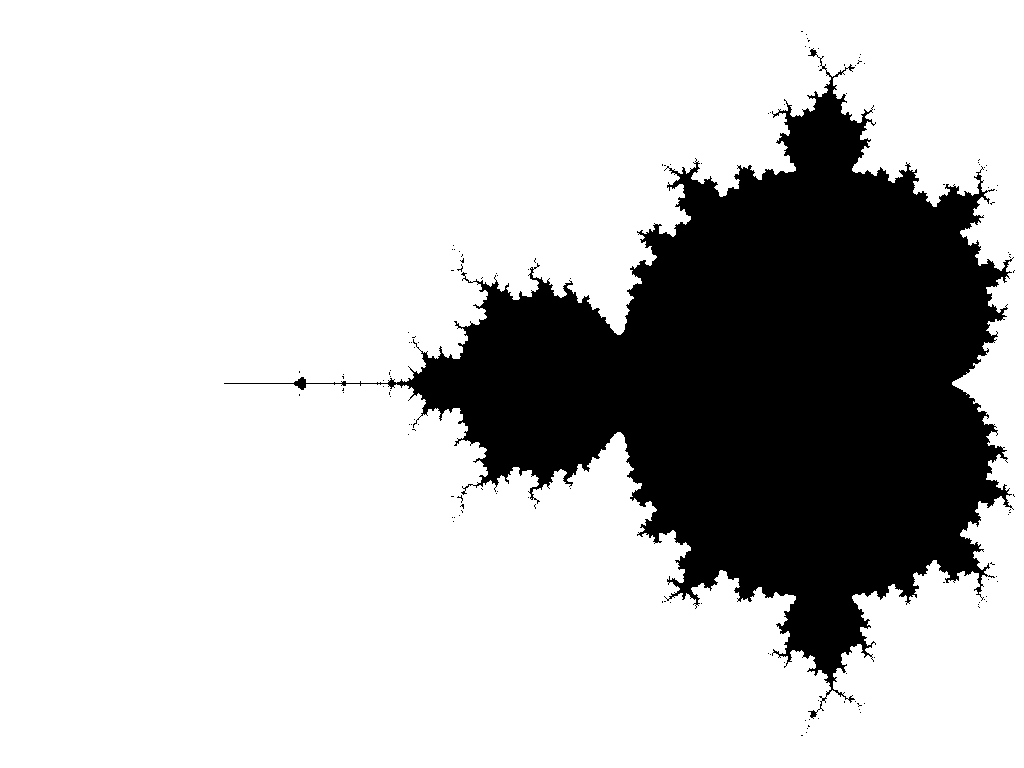
\includegraphics[width=\textwidth]{figures/Mandelbrot_black.png}
  \end{columns}
\end{frame}

%% ==================================================================== 4
\begin{frame}{CPU renderer: skalarna varijanta i SIMD}
  \begin{columns}[T]
    \column{0.46\textwidth}
      \begin{itemize}
        \item \code{f64} + FMA, test bekstva kao $|z_n|^2>4$
        \item Brentova detekcija ciklusa prepoznaje periodične piksele bez čekanja na \code{max\_iter}
        \item SIMD: \code{f32x8} / \code{f64x4} + maska aktivnih traka; dva nezavisna lanca za ILP
      \end{itemize}
      \vspace{0.4em}
      {\color{accent}\bfseries do $2.4\times$ ubrzanje} nad skalarnom osnovom
    \column{0.5\textwidth}
      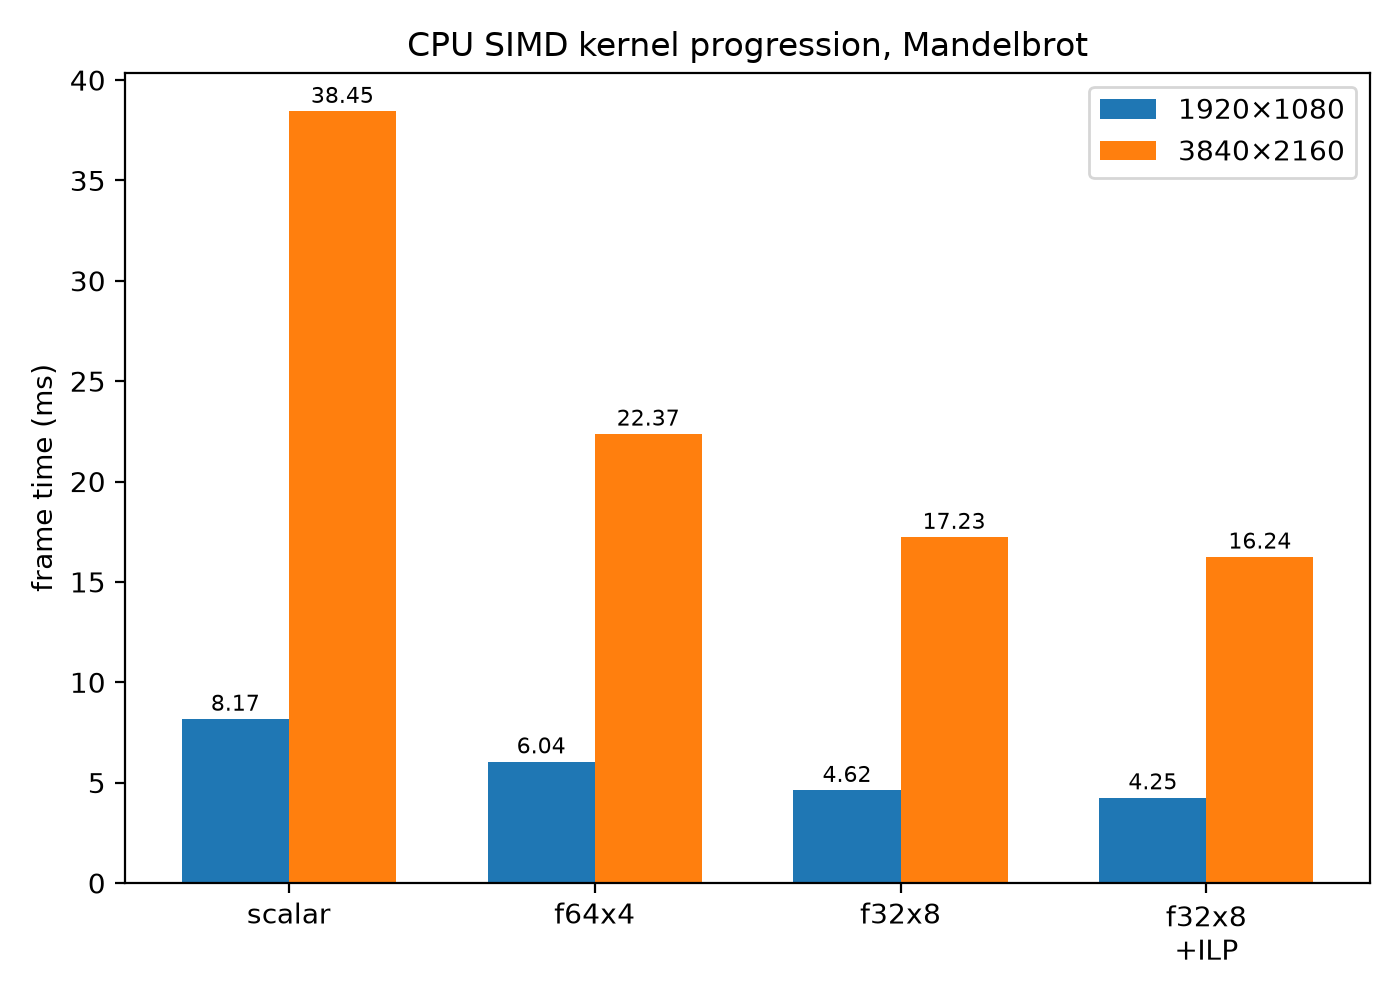
\includegraphics[width=\textwidth]{figures/results-simd-progression.png}
  \end{columns}
\end{frame}

%% ==================================================================== 5
\begin{frame}{Rani izlazak, Mariani-Silver, procena rastojanja}
  \begin{columns}[c]
    \column{0.46\textwidth}
      \begin{itemize}
        \item Kardioida i period-2 balon: tačan zatvoren oblik, bez iteracije
        \item Mariani-Silver: testira se samo ivica pravougaonika; ako je uniformna, popunjava se bez računanja unutrašnjosti
        \item Procena rastojanja (DEM): meri koliko je piksel daleko od granice, koristi se kao dodatni test odsecanja
      \end{itemize}
    \column{0.46\textwidth}
      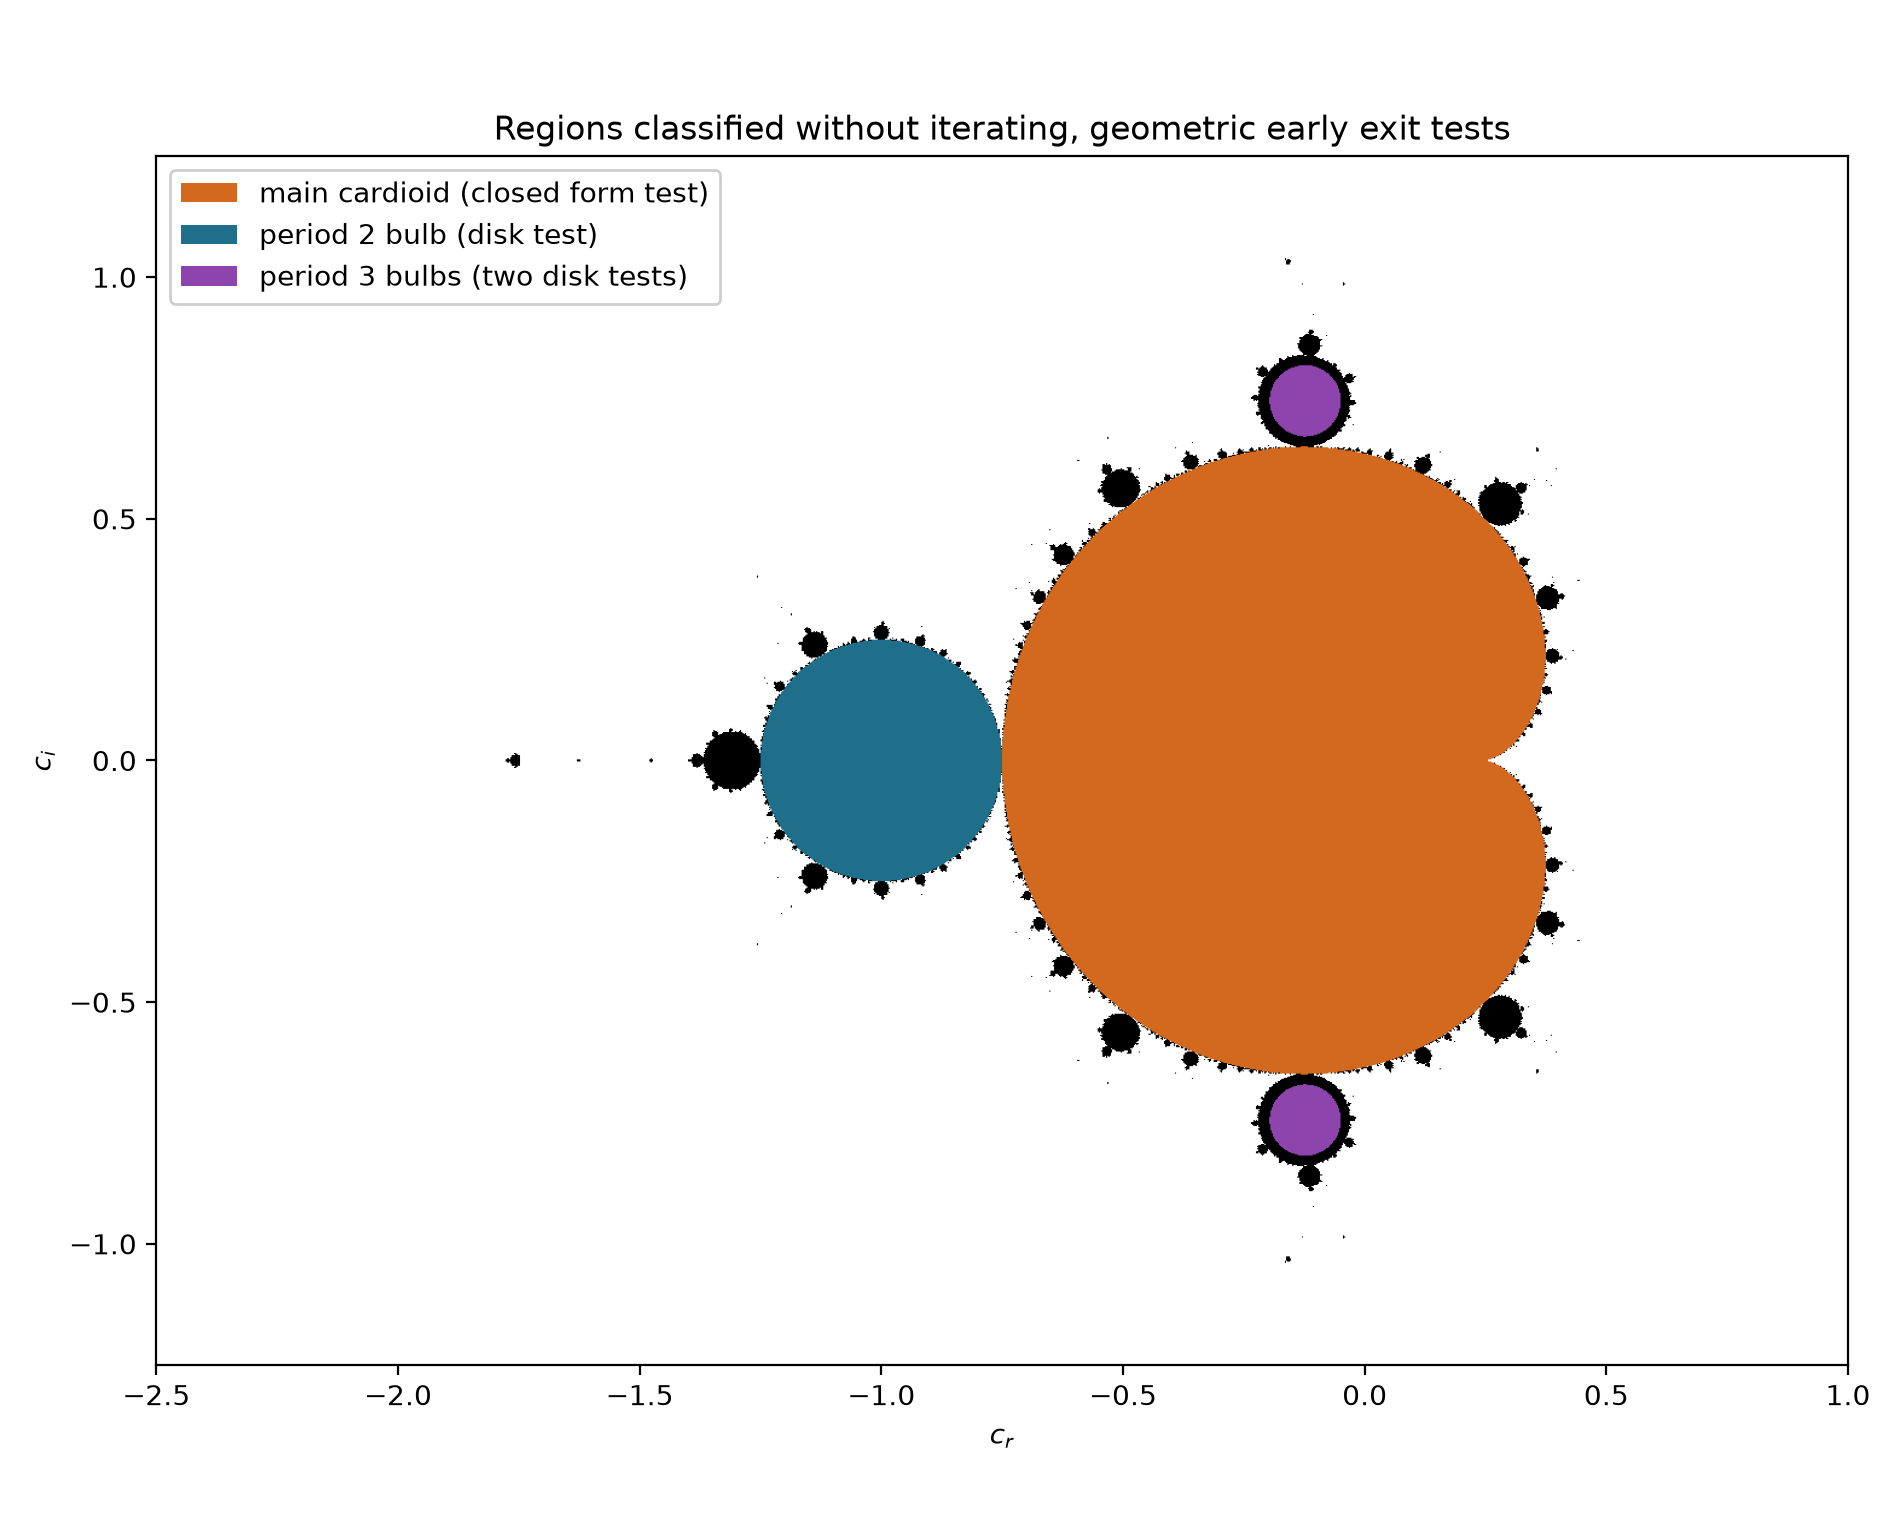
\includegraphics[width=\textwidth]{figures/alg-early-exit-regions.png}
  \end{columns}
\end{frame}

%% ==================================================================== 6
\begin{frame}{Duboki zum i neočekivani rezultati}
  \begin{itemize}
    \item \textbf{Teorija perturbacije} ($\delta_n = z_n - Z_n$, rebasing, do 8 referenci) + \code{double-double} referentna orbita za zum $>10^{12}$
    \item[]
    \item Dve optimizacije koje \textbf{nisu} isplatile na ovom hardveru:
    \begin{itemize}
      \item perturbacija ne donosi dobitak do zuma $10^{12}$ (\code{f64} je dovoljan)
      \item Hilbertova kriva (CPU obilazak) je \emph{sporija} od reda po redovima
    \end{itemize}
  \end{itemize}
  \vspace{0.5em}
\end{frame}

%% ==================================================================== 7
\begin{frame}{GPU implementacija: WebGPU i CUDA}
  \begin{itemize}
    \item \textbf{WebGPU} (\code{wgpu}) kompajlira se u Vulkan, Metal ili DirectX preko drajvera; WGSL nema \code{f64}, pa je kernel isključivo \code{f32}
    \item Isti WGSL kernel deli sve tipove fraktala; dve ulazne tačke: ceo kadar (radne grupe $16{\times}16$) i pojedinačne pločice za hibridni raspoređivač
    \item \textbf{CUDA} cilja \code{sm\_86} (Ampere); PTX se kompajlira unapred pomoću \code{nvcc}, bez kompajliranja u realnom vremenu
    \item CUDA zadržava pun \code{f64} paritet sa CPU-om; \code{--ftz=false} čuva denormalizovane brojeve, potrebne za tačnost glatkog bojenja blizu praga bekstva
  \end{itemize}
  \vspace{0.3em}
  \begin{center}
  \small
  \begin{tabular}{lcc}
    \toprule
     & \textbf{WebGPU} & \textbf{CUDA} \\
    \midrule
    prenosivost & Vulkan / Metal / DirectX & samo NVIDIA \\
    preciznost & samo \code{f32} & \code{f32} i \code{f64} \\
    kompajliranje & WGSL, u realnom vremenu & PTX, unapred (\code{nvcc}) \\
    kadar (1080p, zum 1) & $2.26$ ms & $1.61$ ms \\
    \bottomrule
  \end{tabular}
  \end{center}
\end{frame}

%% ==================================================================== 7b
\begin{frame}{GPU optimizacije}
  \begin{itemize}
    \item \code{--fmad=false} isključuje sažimanje množenja i sabiranja, pa CUDA zaokružuje bit-identično sa CPU kernelom
    \item \code{colorize()} premešten na GPU (histogram + očitavanje iz palete kao poseban kernel), tačno do piksela u odnosu na CPU verziju
    \item Mortonov (Z) redosled niti, isproban za bolju lokalnost unutar \emph{warp}-a, donosi samo $+1{,}9\%$, u granicama šuma
  \end{itemize}
  \vspace{0.3em}
  \begin{center}
    {\color{accent}\bfseries colorize na GPU-u: $54$--$63\%$ brže od početka do kraja} \\
    {\small\color{graytext} pri plitkim i srednjim uvećanjima, gde je bojenje ranije dominiralo kadrom}
  \end{center}
\end{frame}

%% ==================================================================== 7c
\begin{frame}{Usko grlo: PCIe magistrala}
  \begin{columns}[T]
    \column{0.46\textwidth}
      \begin{itemize}
        \item Diskretni GPU je dostupan samo preko \textbf{PCIe 3.0 x8} ($\sim\!7.9$ GB/s teorijski)
        \item Integrisani GPU deli sistemsku RAM sa CPU-om, bez PCIe prenosa
        \item Kadar $1920{\times}1080$ = $8.29$ MB koji se prenosi nazad na \emph{svaki} kadar
        \item \emph{Pinned memory} omogućava DMA direktno u bafer pozivaoca
      \end{itemize}
    \column{0.5\textwidth}
      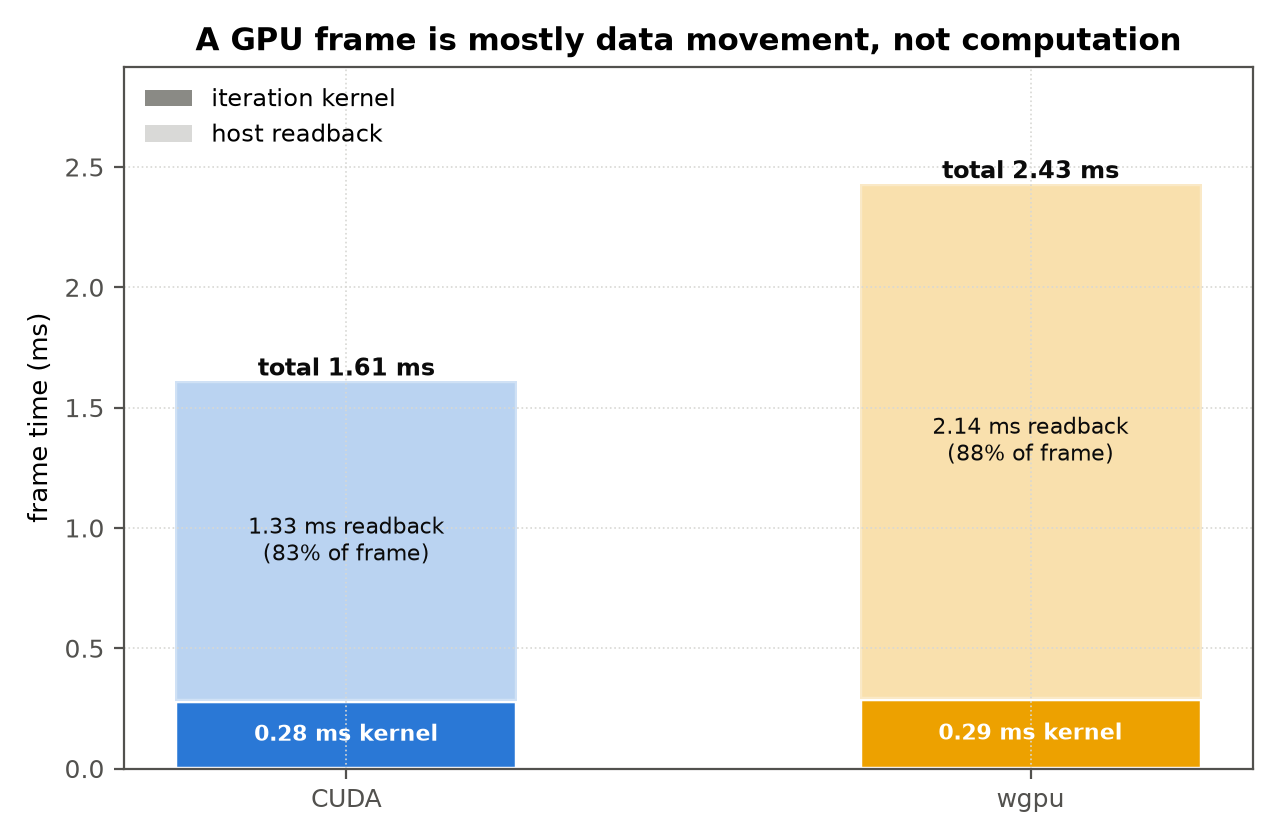
\includegraphics[width=\textwidth]{figures/results-gpu-frame-breakdown.png}
  \end{columns}
  \vspace{0.3em}
  \begin{center}
    {\large\color{accentwarm}\bfseries $80$--$90\%$ vremena GPU kadra je prenos}
  \end{center}
\end{frame}

%% ==================================================================== 8
\begin{frame}{Hibridni CPU+GPU raspoređivač}
  \begin{columns}[T]
    \column{0.48\textwidth}
      \textbf{Zašto:}
      \begin{itemize}
        \item GPU niti rade u \emph{warp}-ovima od 32, u lok-koraku, pa jedan spor piksel usporava ceo \emph{warp}
        \item CPU nit je nezavisna, pa su divergentne granične oblasti jeftinije na CPU-u
      \end{itemize}
    \column{0.48\textwidth}
      \textbf{Dizajn (4 koraka):}
      \begin{enumerate}
        \item klasifikacija pločica (4 temena)
        \item raspodela: GPU odmah, CPU iz reda
        \item krađa posla unutar kadra
        \item PI regulator između kadrova
      \end{enumerate}
  \end{columns}
\end{frame}

%% ==================================================================== 9
\begin{frame}{Klasifikacija pločica i PI regulator}
  \begin{columns}[c]
    \column{0.42\textwidth}
      \[
        s=\frac{\max(i_k)-\min(i_k)}{N}
      \]
      \[
        \text{threshold} \,{-}{=}\, K_P\,\text{err} + K_I\,\overline{\text{err}}
      \]
      \begin{itemize}
        \item $s<$ prag: pločica ide na GPU, inače rekurzivna podela
        \item $\text{err}=t_{\text{gpu}}-t_{\text{cpu}}$, klizni prosek od 16 kadrova
      \end{itemize}
    \column{0.54\textwidth}
      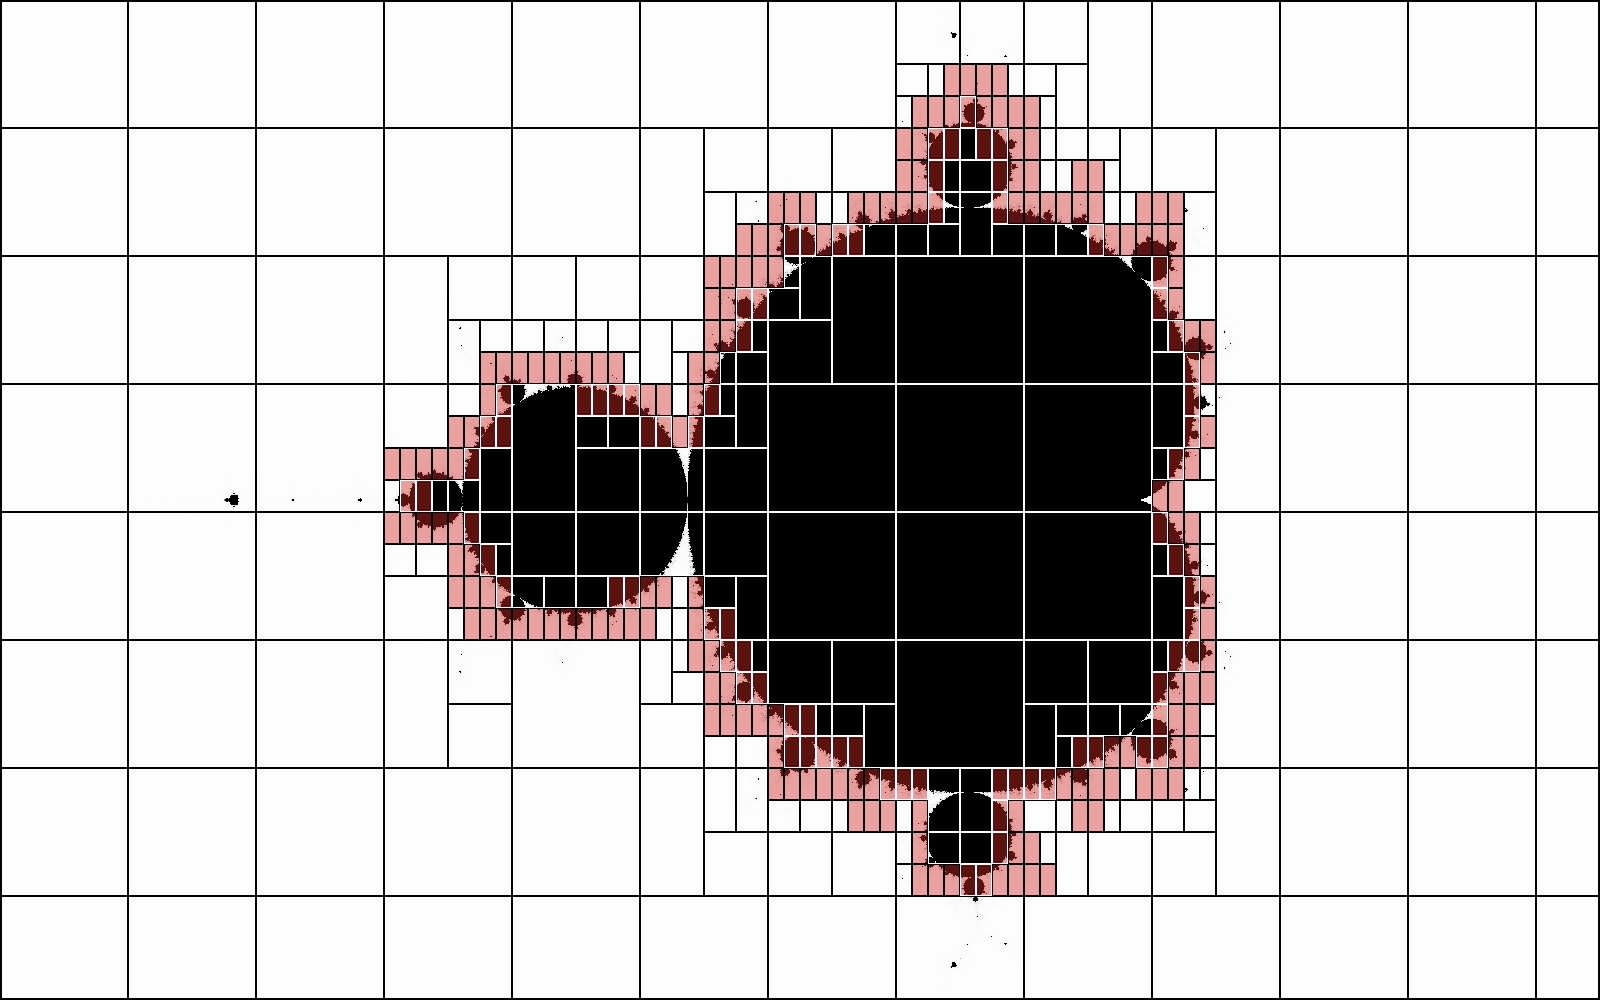
\includegraphics[width=\textwidth]{figures/sched-tiling.png}
  \end{columns}
\end{frame}

%% ==================================================================== 10
\begin{frame}{Rezultati: propusnost renderovanja}
  \begin{center}
    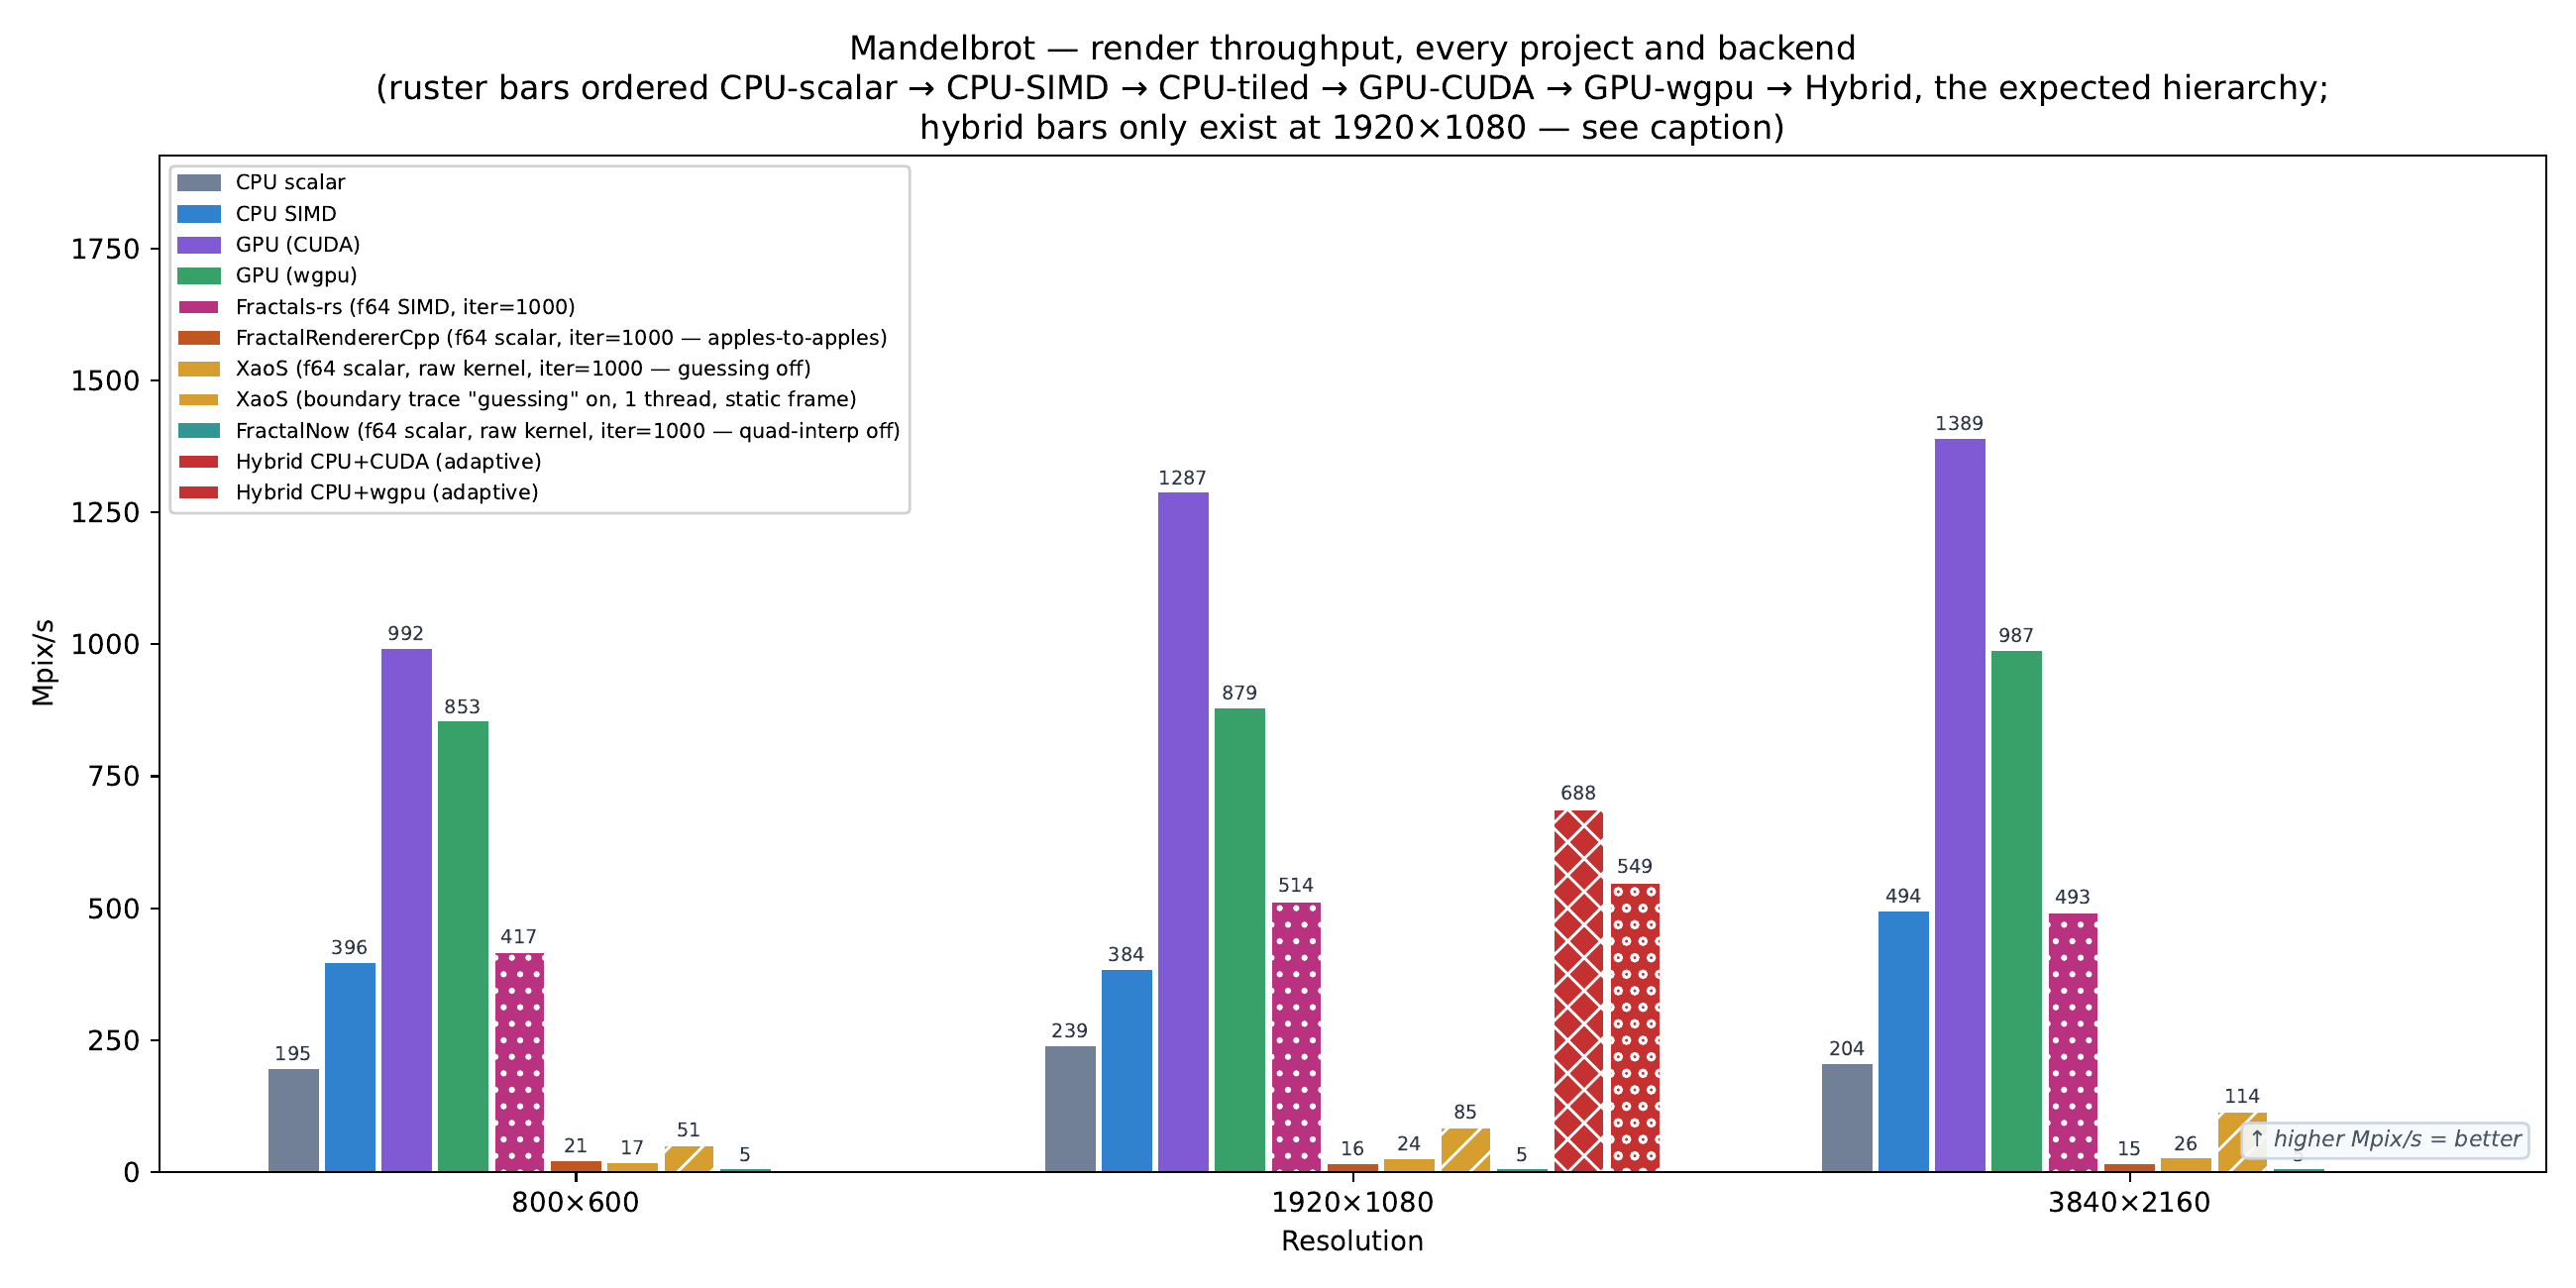
\includegraphics[width=0.78\textwidth,height=0.58\textheight,keepaspectratio]{figures/ruster-throughput-all-backends.png}
  \end{center}
  \begin{center}
    {\color{accent}\bfseries CUDA: $1389$ Mpix/s na 4K} \quad
    {\small\color{graytext} AMD Ryzen 7 5800H + RTX 3050 Laptop, Mandelbrotov skup, \code{max\_iter}=1000}
  \end{center}
\end{frame}

%% ==================================================================== 11
\begin{frame}{Rezultati: raspoređivač pri plitkom zumu}
  \begin{columns}[T]
    \column{0.5\textwidth}
      \centering
      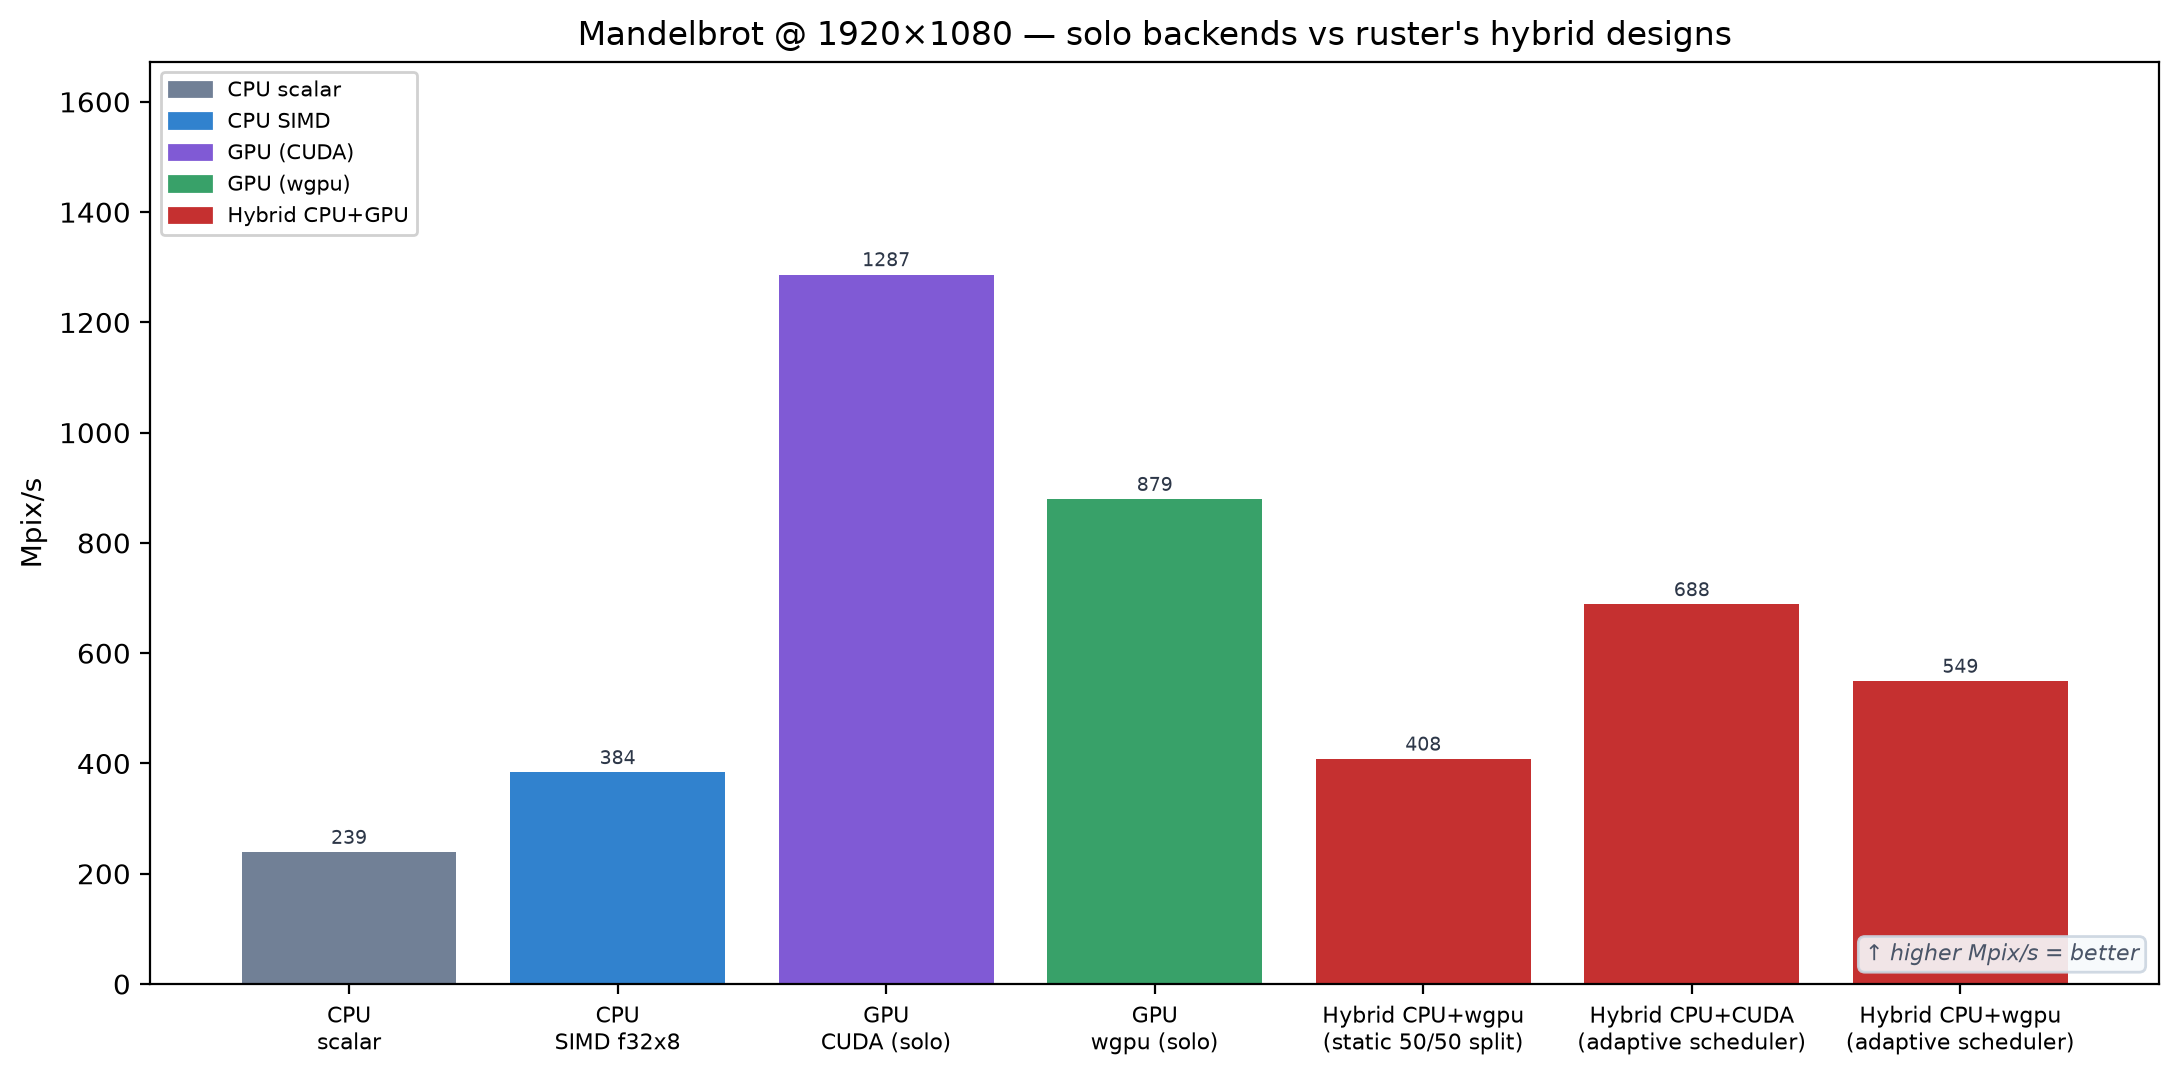
\includegraphics[width=\textwidth,height=0.62\textheight,keepaspectratio]{figures/ruster-solo-vs-hybrid.png}
    \column{0.46\textwidth}
      \vspace{0.5cm}
      \begin{itemize}
        \item Pri plitkom zumu, samostalni GPU je već dovoljno brz i skoro uvek pobeđuje
        \item Raspoređivač tu samo dodaje trošak klasifikacije, bez koristi
      \end{itemize}
      \vspace{0.5em}
      \begin{center}
        {\color{accentwarm}\bfseries gubi od samostalnog GPU-a}\\
        {\scriptsize\color{graytext} nema neravnoteže između uređaja koju bi ispravio}
      \end{center}
  \end{columns}
\end{frame}

%% ==================================================================== 11b
\begin{frame}{Rezultati: raspoređivač pri dubokom zumu}
  \vspace{-0.15cm}
  \begin{columns}[T]
    \column{0.48\textwidth}
      \centering
      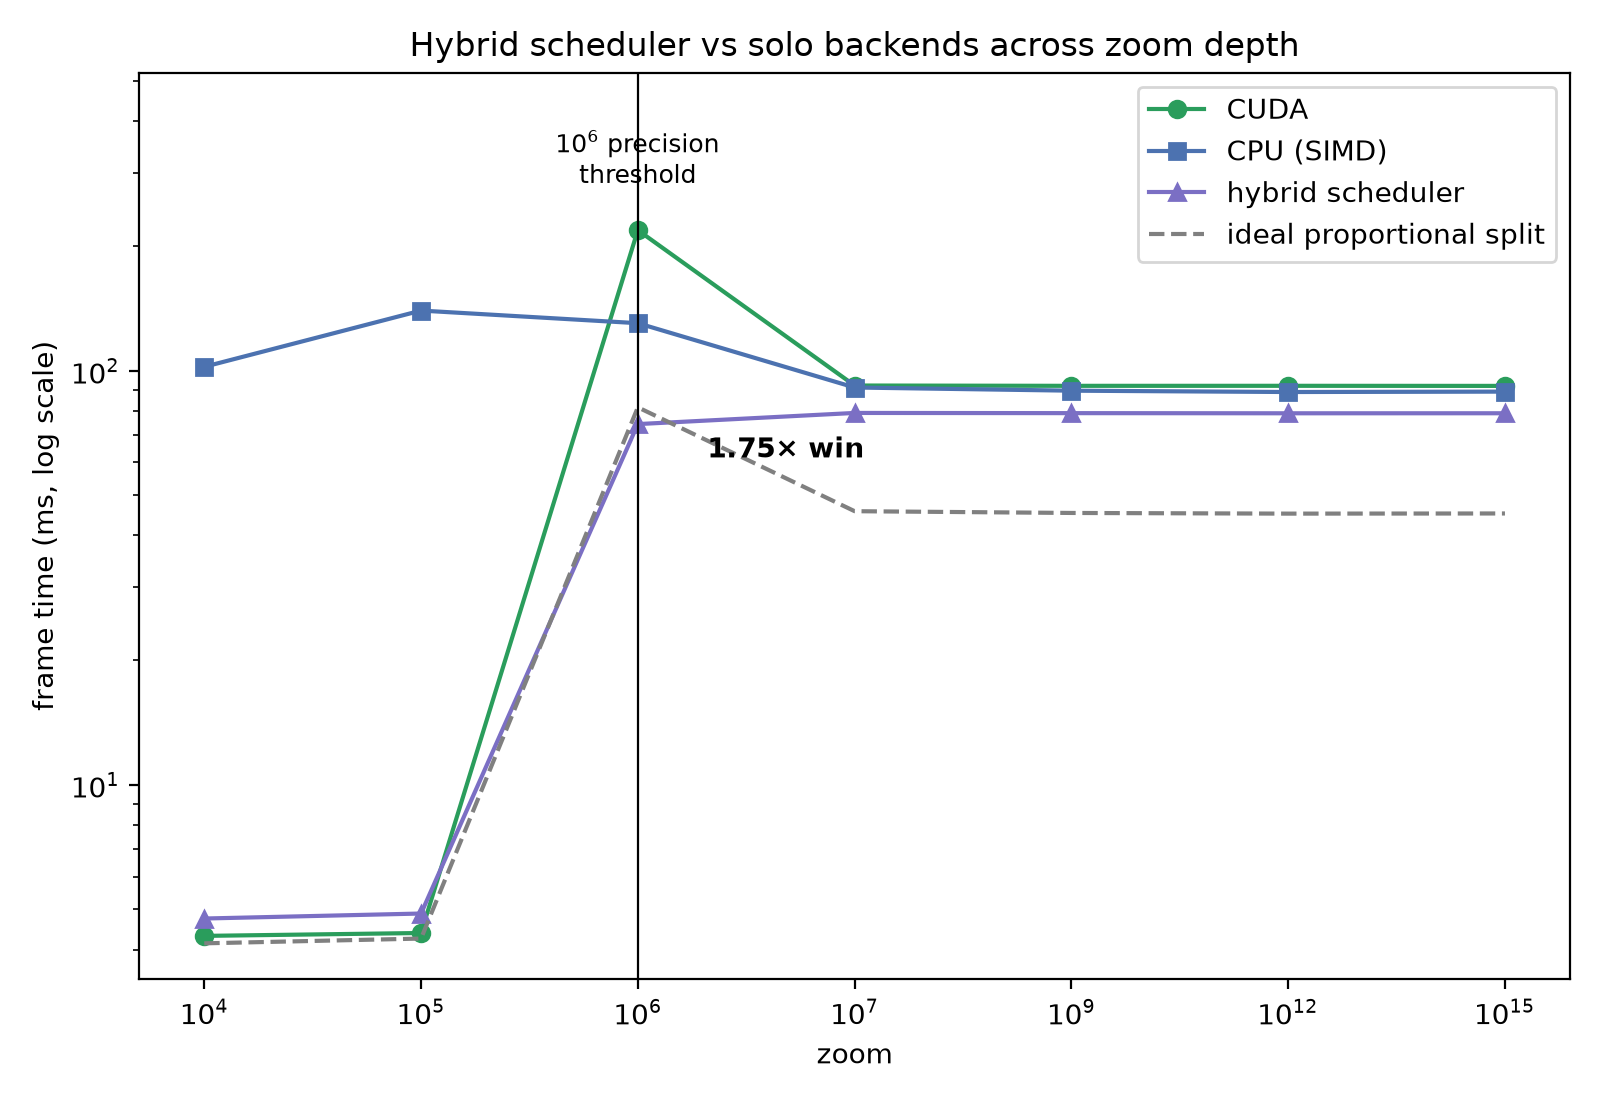
\includegraphics[width=\textwidth,height=0.5\textheight,keepaspectratio]{figures/results-scheduler-deepzoom.png}\\[0.3em]
      {\scriptsize\color{graytext} Na pragu preciznosti $10^6$ GPU prelazi na sporiju \code{f64} aritmetiku, pa CPU postaje brži solo uređaj}
    \column{0.46\textwidth}
      \vspace{0.3cm}
      \centering
      \small
      \begin{tabular}{lr}
        \toprule
        konfiguracija & vreme \\
        \midrule
        CPU (solo) & $130$ ms \\
        "idealna" podela & $81.6$ ms \\
        \textbf{hibrid} & \textbf{$74.3$ ms} \\
        \bottomrule
      \end{tabular}
      \vspace{0.45em}

      {\large\color{accent}\bfseries $1.75\times$} {\small brže od CPU-a}\\[0.25em]
      {\large\color{accentlight}\bfseries $1.10\times$} {\small brže od "idealne" podele}
  \end{columns}
  \vspace{0.35em}
  {\scriptsize\color{graytext} "Idealna" podela samo deli posao proporcionalno izmerenoj brzini uređaja, pod pretpostavkom da je
  svaki piksel podjednako skup. Stvarna granica skupa mnogo je skuplja od unutrašnjosti; klasifikator pločica to
  prepoznaje i usmerava skupe delove ka boljem uređaju, pa hibrid nadmašuje čak i tu "idealnu" podelu.}
\end{frame}

%% ==================================================================== 12
\begin{frame}{Poređenje sa drugim rendererima i validacija}
  \begin{columns}[T]
    \column{0.5\textwidth}
      \centering
      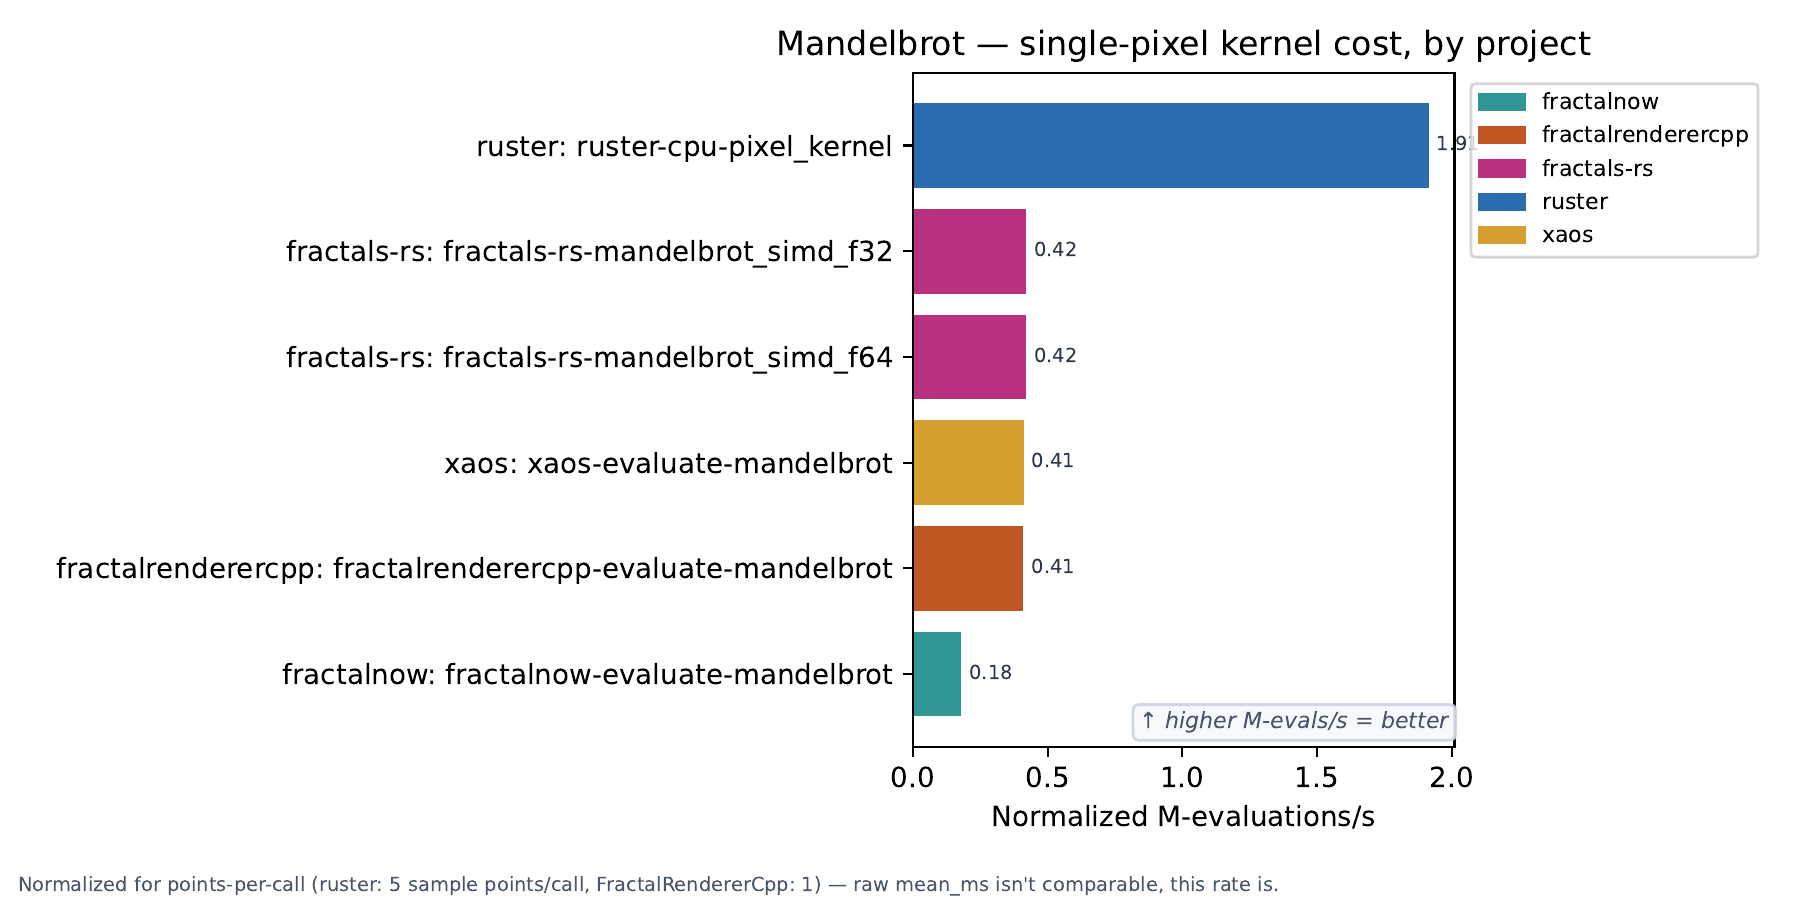
\includegraphics[width=\textwidth,height=0.52\textheight,keepaspectratio]{figures/ruster-pixel-kernel-cost.png}\\[0.3em]
      {\scriptsize\color{graytext} Trošak samog kernela po pikselu (miliona evaluacija/s, normalizovano), bez niti, bojenja i "nagađanja" kod XaoS-a i FractalNow-a: ruster je red veličine brži od najbržeg konkurenta, dva reda od najsporijeg}
    \column{0.46\textwidth}
      \centering
      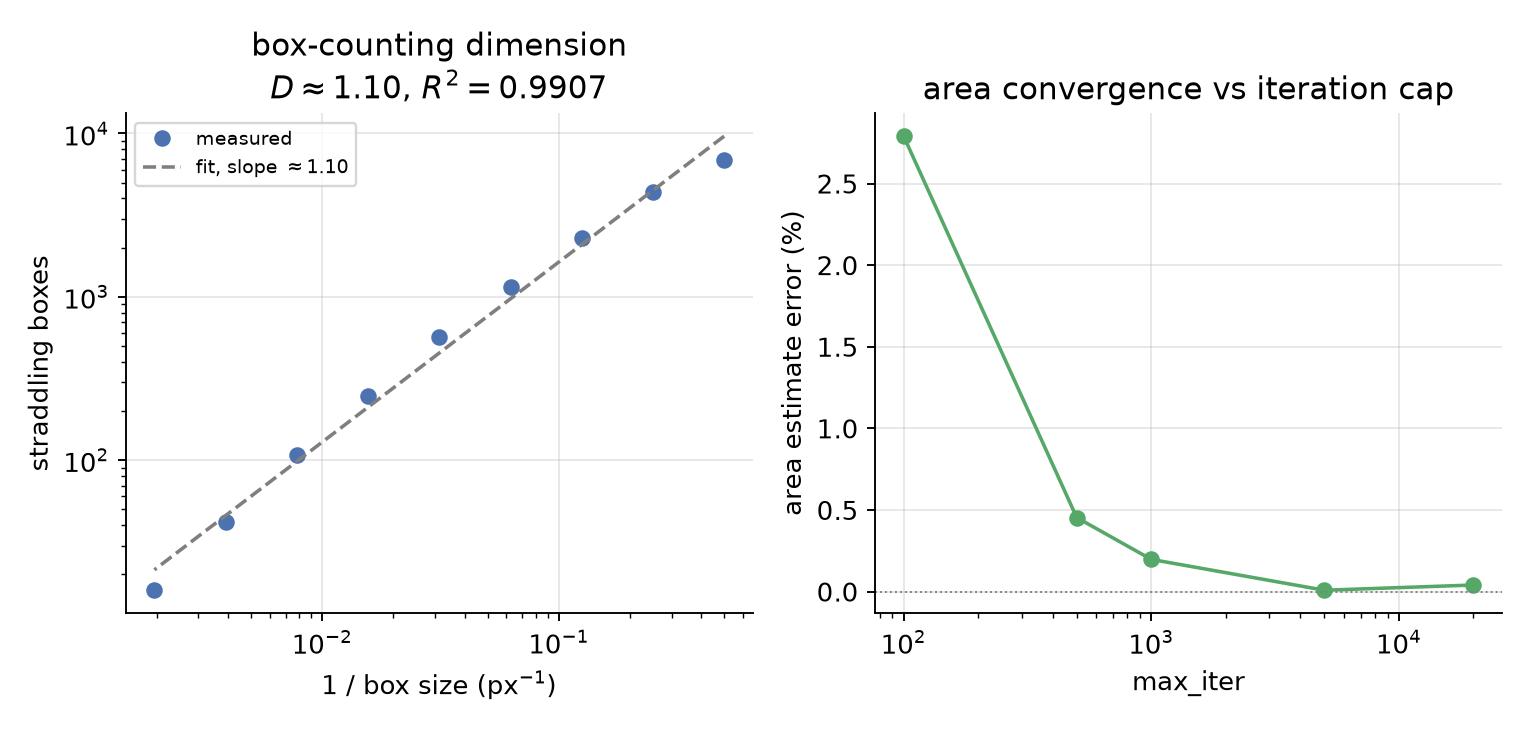
\includegraphics[width=\textwidth,height=0.52\textheight,keepaspectratio]{figures/results-numerical-validation.png}\\[0.3em]
      {\scriptsize\color{graytext} Box-counting dimenzija $\approx1.10$; konvergencija površine ka $1.50659177$}
  \end{columns}
  \vspace{0.4em}
\end{frame}

%% ==================================================================== 13
\begin{frame}{Zaključak}
  \begin{itemize}
    \item \textbf{CPU strana važnija nego očekivano}: rani izlazak i detekcija ciklusa daju $\sim\!16\times$ nad naivnim C++ rendererom, bez GPU-a
    \item \textbf{GPU dominira transferom i bojenjem, ne kernelom}: premeštanje bojenja na uređaj je najveći pojedinačni dobitak
    \item \textbf{Raspoređivač se isplati tačno na pragu preciznosti}, gubi kad su uređaji neuravnoteženi
  \end{itemize}
  \vspace{0.5em}
  {\scriptsize\color{graytext} Budući rad: \code{colorize()} na GPU za wgpu i hibrid; podešavanje raspoređivača na dubokom zumu; perturbacija na stvarno dubokim zumovima; poređenje sa novim GPU-konkurentnim rešenjem koje je nedavno objavio jedan poznati render fraktala.}
\end{frame}

%% ==================================================================== 14
\begin{frame}[plain]
  \vspace{2.0cm}
  \begin{center}
    {\usebeamerfont{title}\color{accent} Hvala na pažnji}\\[1.2em]
    {\color{accent}\rule{0.12\textwidth}{2pt}}\\[1.2em]
    {\large\color{graytext} Pitanja?}
  \end{center}
\end{frame}

\end{document}
